\documentclass[11pt]{article}
\usepackage[margin=1in]{geometry}
\usepackage{amsmath,amssymb}
\usepackage{graphicx}
\usepackage{color}
\usepackage{xcolor}
\usepackage{adjustbox} 
\usepackage{setspace}
\usepackage{booktabs}
\usepackage{rotating}
\usepackage{indentfirst}
\usepackage{natbib,subfig}
\setcitestyle{maxcitenames=10, maxbibnames=10}
\usepackage{enumitem}
\usepackage{gensymb}
\usepackage[normalem]{ulem}
\usepackage{xcolor}
\usepackage[english]{babel}
\usepackage{amsthm}
\usepackage{bbm}
\usepackage{fancyhdr}
\usepackage{bbding}

\usepackage{pdfpages}
\usepackage[colorlinks=true, linkcolor=blue, citecolor=black, filecolor=black, urlcolor=blue]{hyperref}

% At the beginning of your document
\usepackage{xstring}


\bibliographystyle{apalike}
\onehalfspacing
\title{Healthcare amenities, housing prices and senior migration}
\author{Jeffrey Ohl}
\date{June 4 2025}


\begin{document}
\maketitle

\section{Reminder of the research areas}
Two broad classes of ideas:

\begin{enumerate}
\item How are healthcare amenities capitalized into housing prices? 
\item How does senior migration drive up housing prices? If so, is  healthcare quality a primary force attracting them? Are cities doing anything to try to attract seniors?
\end{enumerate}


\section{Suggestions from last meeting / Summary of what I've done since last time}
\begin{enumerate}
    \item Read: 
\begin{itemize}
\item Read \cite{AlexanderRichards2023}, on the effects of rural hospital closures. Done. 
\item Check out Mathilde Mu\~noz recent work to get an idea of what has been done already: \citep{KalinLevyMunoz2024} on international migration, and \citep{BadillaMarotoFaberLevyMunoz2024}, on domestic migration in France. Done, see discussion below. 
\item Two papers on how much people value healthcare: \citep{FinkelsteinHendrenLuttmer2019} and \citep{FinkelsteinHendrenShepard2019} - Still need to do this.
\end{itemize}

\item Institutional details and anecdata to collect:
\begin{itemize}
    \item Is anyone saying they will retire to any of the Mayo Clinic locations (including Florida and Arizona locations)? - Yes, some evidence of this below. 
\item Is Mayo Clinic trying to build more housing for their people? - See below. 

\item How have house prices moved in Rochester since the 2013 announcement of DMC?  - See below. 
\end{itemize}


\item Statistical analyses:
\begin{itemize}
\item How did age composition (share 65+) change in places with (high HC vs low HC initial shares), which lost manufacturing? In other words, did having high initial health shares buffer the potential losses induced by manufacturing declines? See below. 
\item How are house prices being influenced by rural hospital closures (basically a slight extension of \cite{AlexanderRichards2023})? See below. 
\end{itemize} %Note this is basically studying the interaction's effect on the age share. %Please pull all data using APIs and analyze this with simple regression (OLS) if you can. %  \textcolor{red}{super concrete .. simpler first pass way to check if HC changed the share of old people who live here  ... WHY ARE we doing this by Manufacturing Loss though? Why not just look at the effect in general, not just for places that lost manufacturing? }



\end{enumerate}



\section{Institutional details }

\subsection{How do people choose where to retire?}
A survey by the insurance company, TransAmerica, listed the following top factors seniors reported considering when choosing where to retire:  affordable cost of living (65\%); proximity to family and friends (61\%); access to quality health care (49\%); low crime rates (48\%); and good weather (42\%). This is consistent with evidence from  \citep{BadillaMarotoFaberLevyMunoz2024}, that pensioners tend to move to poorer areas. A stylized fact from that paper is that only the lower 2/3 of cantons, by GDP per capita, have net inflows of pensioners. 


Also a fun fact is Mayo Clinic operates its own retirement \href{https://charterhouse-mayo.org/?utm_source=chatgpt.com}{home}.% The senior living apartment complexes are located in mayo clinic. 


%A forum about other examples \href{https://connect.mayoclinic.org/discussion/where-do-you-want-to-grow-old/?pg=26}{source}

\subsection*{Effect of Mayo Clinic build out on house prices (in Rochester)}
We discussed trying to see if large build-outs, like the Destination Medical Center in Rochester, MN (which began in 2013), might have had an effect on house prices. I haven't run the DiD, but Rochester does not appear to show much of a differential gain relative to intuitive control groups. For such a gradual roll-out, identification seems tricky, as we discussed.

%A friend who is from Rochester, MN says that it's commonly accepted that Destination Medical  Center increased existing residents' house values, bu
\begin{figure}[htbp]
    \centering
    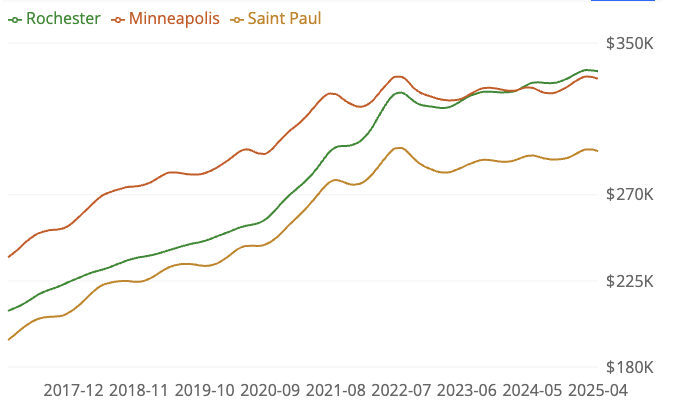
\includegraphics[width=0.9\textwidth]{Rochester.png}
    \caption{House prices in Rochester, MN, relative to Minneapolis, MN and St. Paul, MN,  from 2017-2025. Source: Zillow Home Value Index. }
    \label{fig:rochester_house_prices}
\end{figure}


\subsection*{Is Mayo Clinic building out housing for its workers?}
We discussed this question because the Destination Medical Center build-out has likely increased the number of jobs, and thus demand for housing, quite a lot in Rochester. 

The answer: Not directly, though they are giving money to local groups, some of which support housing. This seemed to me more like surplus sharing to keep the local populations happy, rather than a direct investment in housing. For example, of the 14.25M dollars they are giving to Rochester, 10M is going to Rochester Public Schools.  The quote below describes the \$22M they spent on communities they have locations in.


\textit{
Mayo Clinic cares for its patients, communities and each other, and Mayo’s Bold. Forward. strategy supports this care through work to Cure, Connect, and Transform healthcare for all. As this strategy successfully unfolds, this year Mayo Clinic is able to invest an additional \$22 million in community organizations addressing pressing needs related to housing, food insecurity, access to healthcare, and safe places for learning and youth enrichment. Mayo Clinic's \$22 million commitment will be distributed to organizations serving Rochester, Jacksonville, Phoenix and various Mayo Clinic Health System locations. }


\section{How did age composition change in places with (high vs. low HC initial shares) that lost manufacturing? }

As a reminder, you suggested I look at whether older folks are moving in at higher rates to high vs. low healthcare places, as an initial test. The specific way you suggested I operationalize this was to see if initial healthcare employment share mediated the effect of manufacturing decline at all. 

Procedure:
\begin{enumerate}
\item Use employment data from county business patterns, and demographic data from census. 

\item Classify  healthcare as: NAICS 62 (Health Care and Social Assistance)
\item Classify manufacturing as:  NAICS 31-33 (Manufacturing),    calculate losses in employment shares from 2000 - 2010.
\item Bucket counties by their quartile of loss of manufacturing share, including those that gained, and plot the bivariate relationship in Figure \ref{fig:age_share_change}.
\end{enumerate}

It does not seem like high initial healthcare shares are positively correlated with changes in the over 65 share.  In fact, there is a robust negative correlation, which makes me worry if this could be mechanical, i.e. the places with lots of healthcare already had a large 65+ share in 2000, and hence didn't have much room to go up. Long differences might not be the right way to think about this, so I also look at cross sectional scatters in the appendix in Figure \eqref{fig:HealthOld2000} and \eqref{fig:HealthOld2010}. These display much more variation in the dependent variable and have the expected positive correlation.



Looking across panels, the main effect of initial healthcare employment is clearly negative. But there is a significant interaction between manufacturing loss and healthcare share, as shown in the corresponding regression in Table \ref{tab:regression_results}.\footnote{The main effect is visualized in Figure \ref{fig:aggregate_health_change}}  Interpretation on this interaction:
\begin{itemize}
    \item \textbf{How does the interaction modify the slope on manufacturing loss?} The more health intensive a county already was in 2000, the less negative the coefficient of losing manufacturing on 65+ share becomes. The sign flips from negative to positive once the initial share is above $\approx$ 0.068, which is of course true for most counties. 
\item \textbf{How does the interaction modify the slope on health employment in 2000?} A county with no manufacturing loss sees a negative association between initial health employment share and subsequent senior-share growth. But if its share of manufacturing employment falls enough - 32 pp or more (so only a very small number of counties) - that association turns positive. 
\end{itemize}




\begin{figure}[htbp]
    \centering
    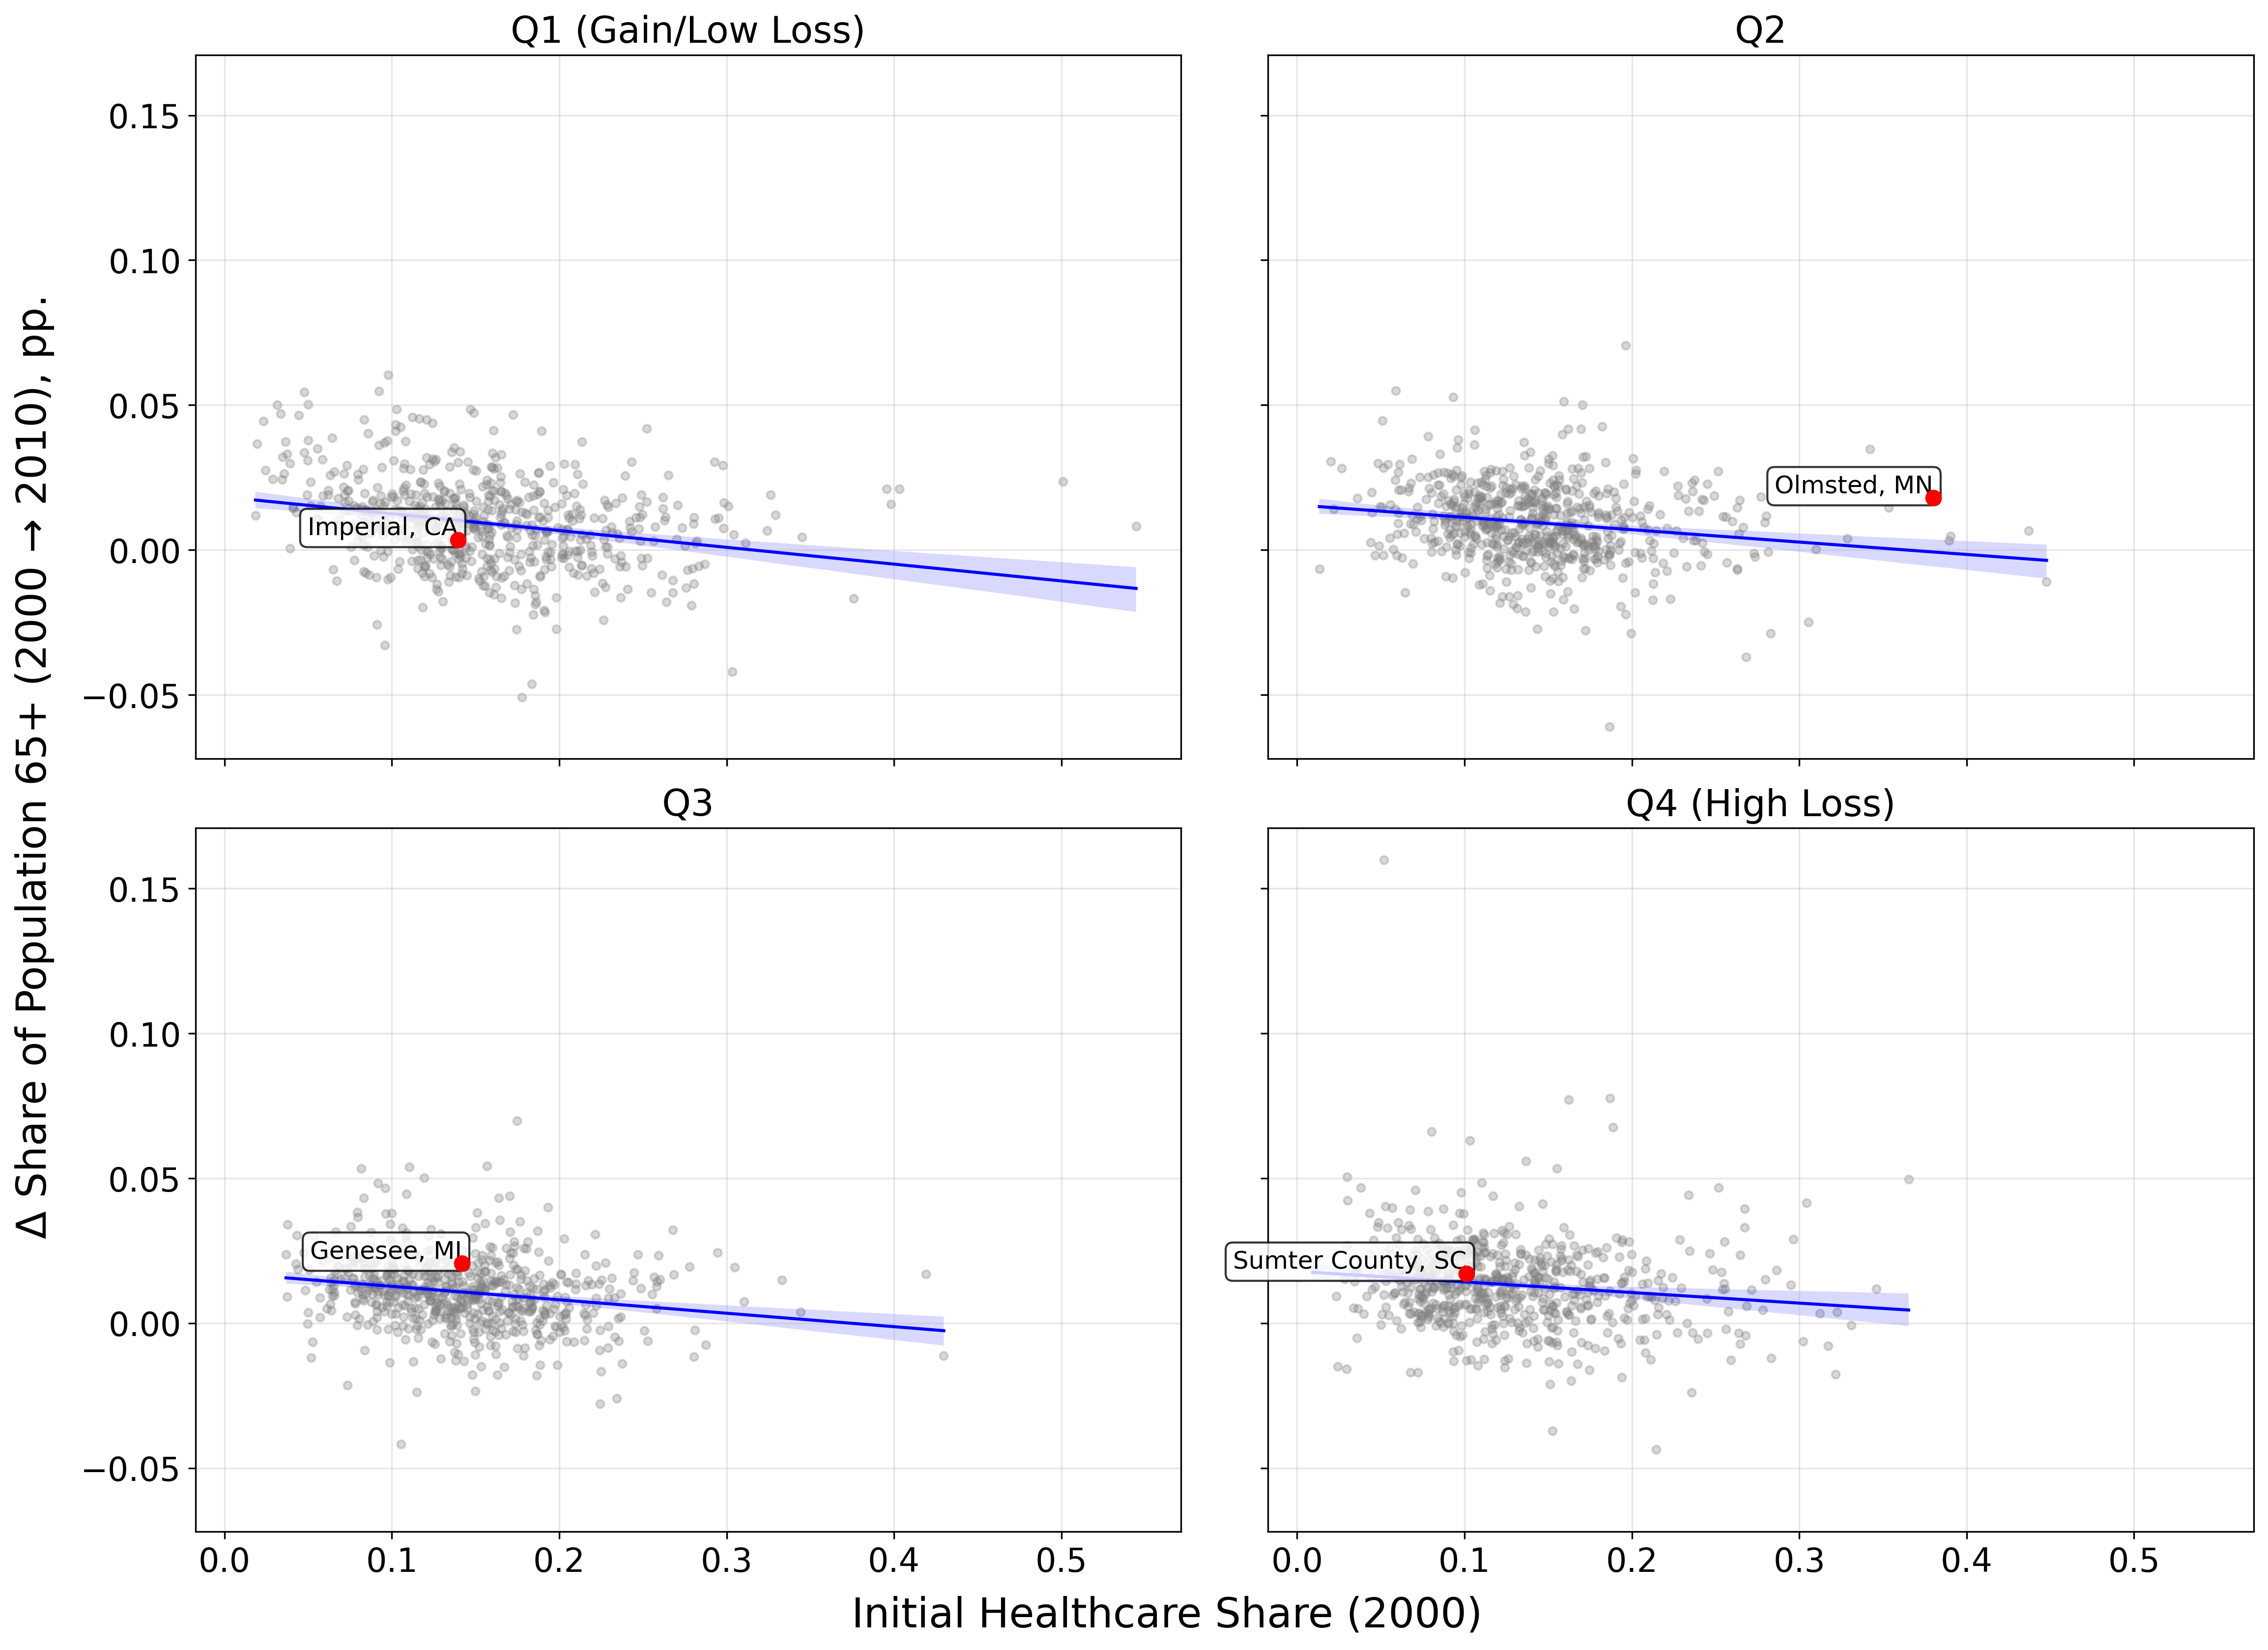
\includegraphics[width=1.15\textwidth]{county_manufacturing_decline_labeled_2000_2010.png}
    \caption{\textit{Panels respond to quartile of manufacturing employment share decline. Y-axis is change in share of population 65+ by county. X-axis is share of employment in healthcare in 2000.  Restricts to counties with non-zero manufacturing and healthcare share in 2000. Changes are from  2000-2010. (CBP and Census)}}
    \label{fig:age_share_change}
\end{figure}



%Note this is basically studying the interaction's effect on the age share. Please pull all data using APIs and analyze this with simple regression (OLS) if you can.   
%\textcolor{red}{super concrete .. simpler first pass way to check if HC changed the share of old people who live here }
%... WHY ARE we doing this by Manufacturing Loss though? Why not just look at the effect in general, not just for places that lost manufacturing?

Which places \textbf{did} become older over this period?  I detail these in the below table; surprisingly to me, Florida doesn't show up, and I can't tell a coherent story from these examples.  For reference, the US as a whole went from 12.4\% to 13.0\% share of population 65+ over this period.

\begin{table}[htbp]
\caption{Top 10 Counties by Increase in Elderly Population Share (2000-2010)}
\label{tab:top10_elderly_increase}
\begin{tabular}{clrrrr}
\toprule
 & County & Pop. (2000) & Pop. (2010) & Pct. 65+ (2000, \%) & $\Delta$ Share 65+ (pp) \\
\midrule
1 & Beaufort County, South Carolina & 120,937 & 162,233 & 15.51 & 4.85 \\
2 & Santa Fe County, New Mexico & 129,292 & 144,170 & 10.75 & 4.37 \\
3 & Livingston County, Michigan & 156,951 & 180,967 & 8.31 & 3.65 \\
4 & Marin County, California & 247,289 & 252,409 & 13.52 & 3.20 \\
5 & Douglas County, Oregon & 100,399 & 107,667 & 17.82 & 3.15 \\
6 & Jefferson County, Colorado & 527,056 & 534,543 & 9.64 & 2.97 \\
7 & Douglas County, Colorado & 175,766 & 285,465 & 4.17 & 2.96 \\
8 & Washington County, Minnesota & 201,130 & 238,136 & 7.59 & 2.90 \\
9 & Mohave County, Arizona & 155,032 & 200,186 & 20.47 & 2.84 \\
10 & Sussex County, New Jersey & 144,166 & 149,265 & 9.12 & 2.84 \\
\bottomrule
\\
\multicolumn{6}{l}{\footnotesize Note: Limited to counties with population $\geq$ 100,000 in 2000.} \\
\end{tabular}
\end{table}



\newpage
\section{Rural hospital closures and house prices}

To get traction on the question of how healthcare amenities are capitalized into housing prices, I start with the extensive margin (going from 1 to 0), following the study of rural hospital closures in \citep{AlexanderRichards2023}.

 I run a staggered DiD and
treat county-quarters as observations. 



\textbf{Disclaimers and overview of data}
\begin{enumerate}
    \item At best, this would tell us the net effect of rural hospital closures on house prices, which includes both employment effects and healthcare amenities, so isn't a very clean test of the mechanism I am interested in. 
\item I am using non-treated counties as a control. The control group used in \citep{AlexanderRichards2023} were all rural counties with no hospital closures, which they licensed from the American Hospital Association.
\item I use the same rural hospital closure data as \citep{AlexanderRichards2023}, from the Sheps Center at UNC. Closure dates are summarized in Figure \ref{fig:closure_dates}.

\item I am using the Zillow Home Value Index for all homes from January 2000 to April 2025, smoothed and seasonally adjusted. This is supposed to be the value of a typical home in the 35th-65th percentile for that county. This is the first time I am using this data, so I still need to check if this is a good measure (e.g. how they are doing the smoothing / seasonal adjustment). 
\end{enumerate}

\subsection*{Empirical Specification}


\begin{enumerate}
\item \textbf{Unit of Observation:} Each observation in the dataset represents a county-quarter pair.
\item \textbf{Treatment Group:} Rural counties that experienced exactly one hospital closure during the sample period. (I drop three counties that experienced multiple)
\item \textbf{Control Group:} All other counties in the US. 

\end{enumerate}






\begin{equation}
ZHVI_{it} = \sum_{q=-4, q \neq -1}^{4} \beta_q \cdot \mathbf{1}(t - t_i^* = q) + \alpha_i + \gamma_t + \epsilon_{it}
\end{equation}

where:
\begin{itemize}
    \item $ZHVI_{it}$ is the Zillow Home Value Index for county $i$ in quarter $t$
    \item $t_i^*$ is the quarter of hospital closure for treated county $i$
    \item $\mathbf{1}(t - t_i^* = q)$ is an indicator equal to 1 if quarter $t$ is $q$ quarters relative to the closure
    \item $\alpha_i$ are county fixed effects
    \item $\gamma_t$ are quarter fixed effects
    %\item $q = -1$ is the omitted reference period
\end{itemize}



The presence of pre-trends, and lack of precision preclude much of an interpretation.  Raw means are shown in appendix Figure \ref{fig:rawmeans}

\begin{figure}[htbp]
\centering
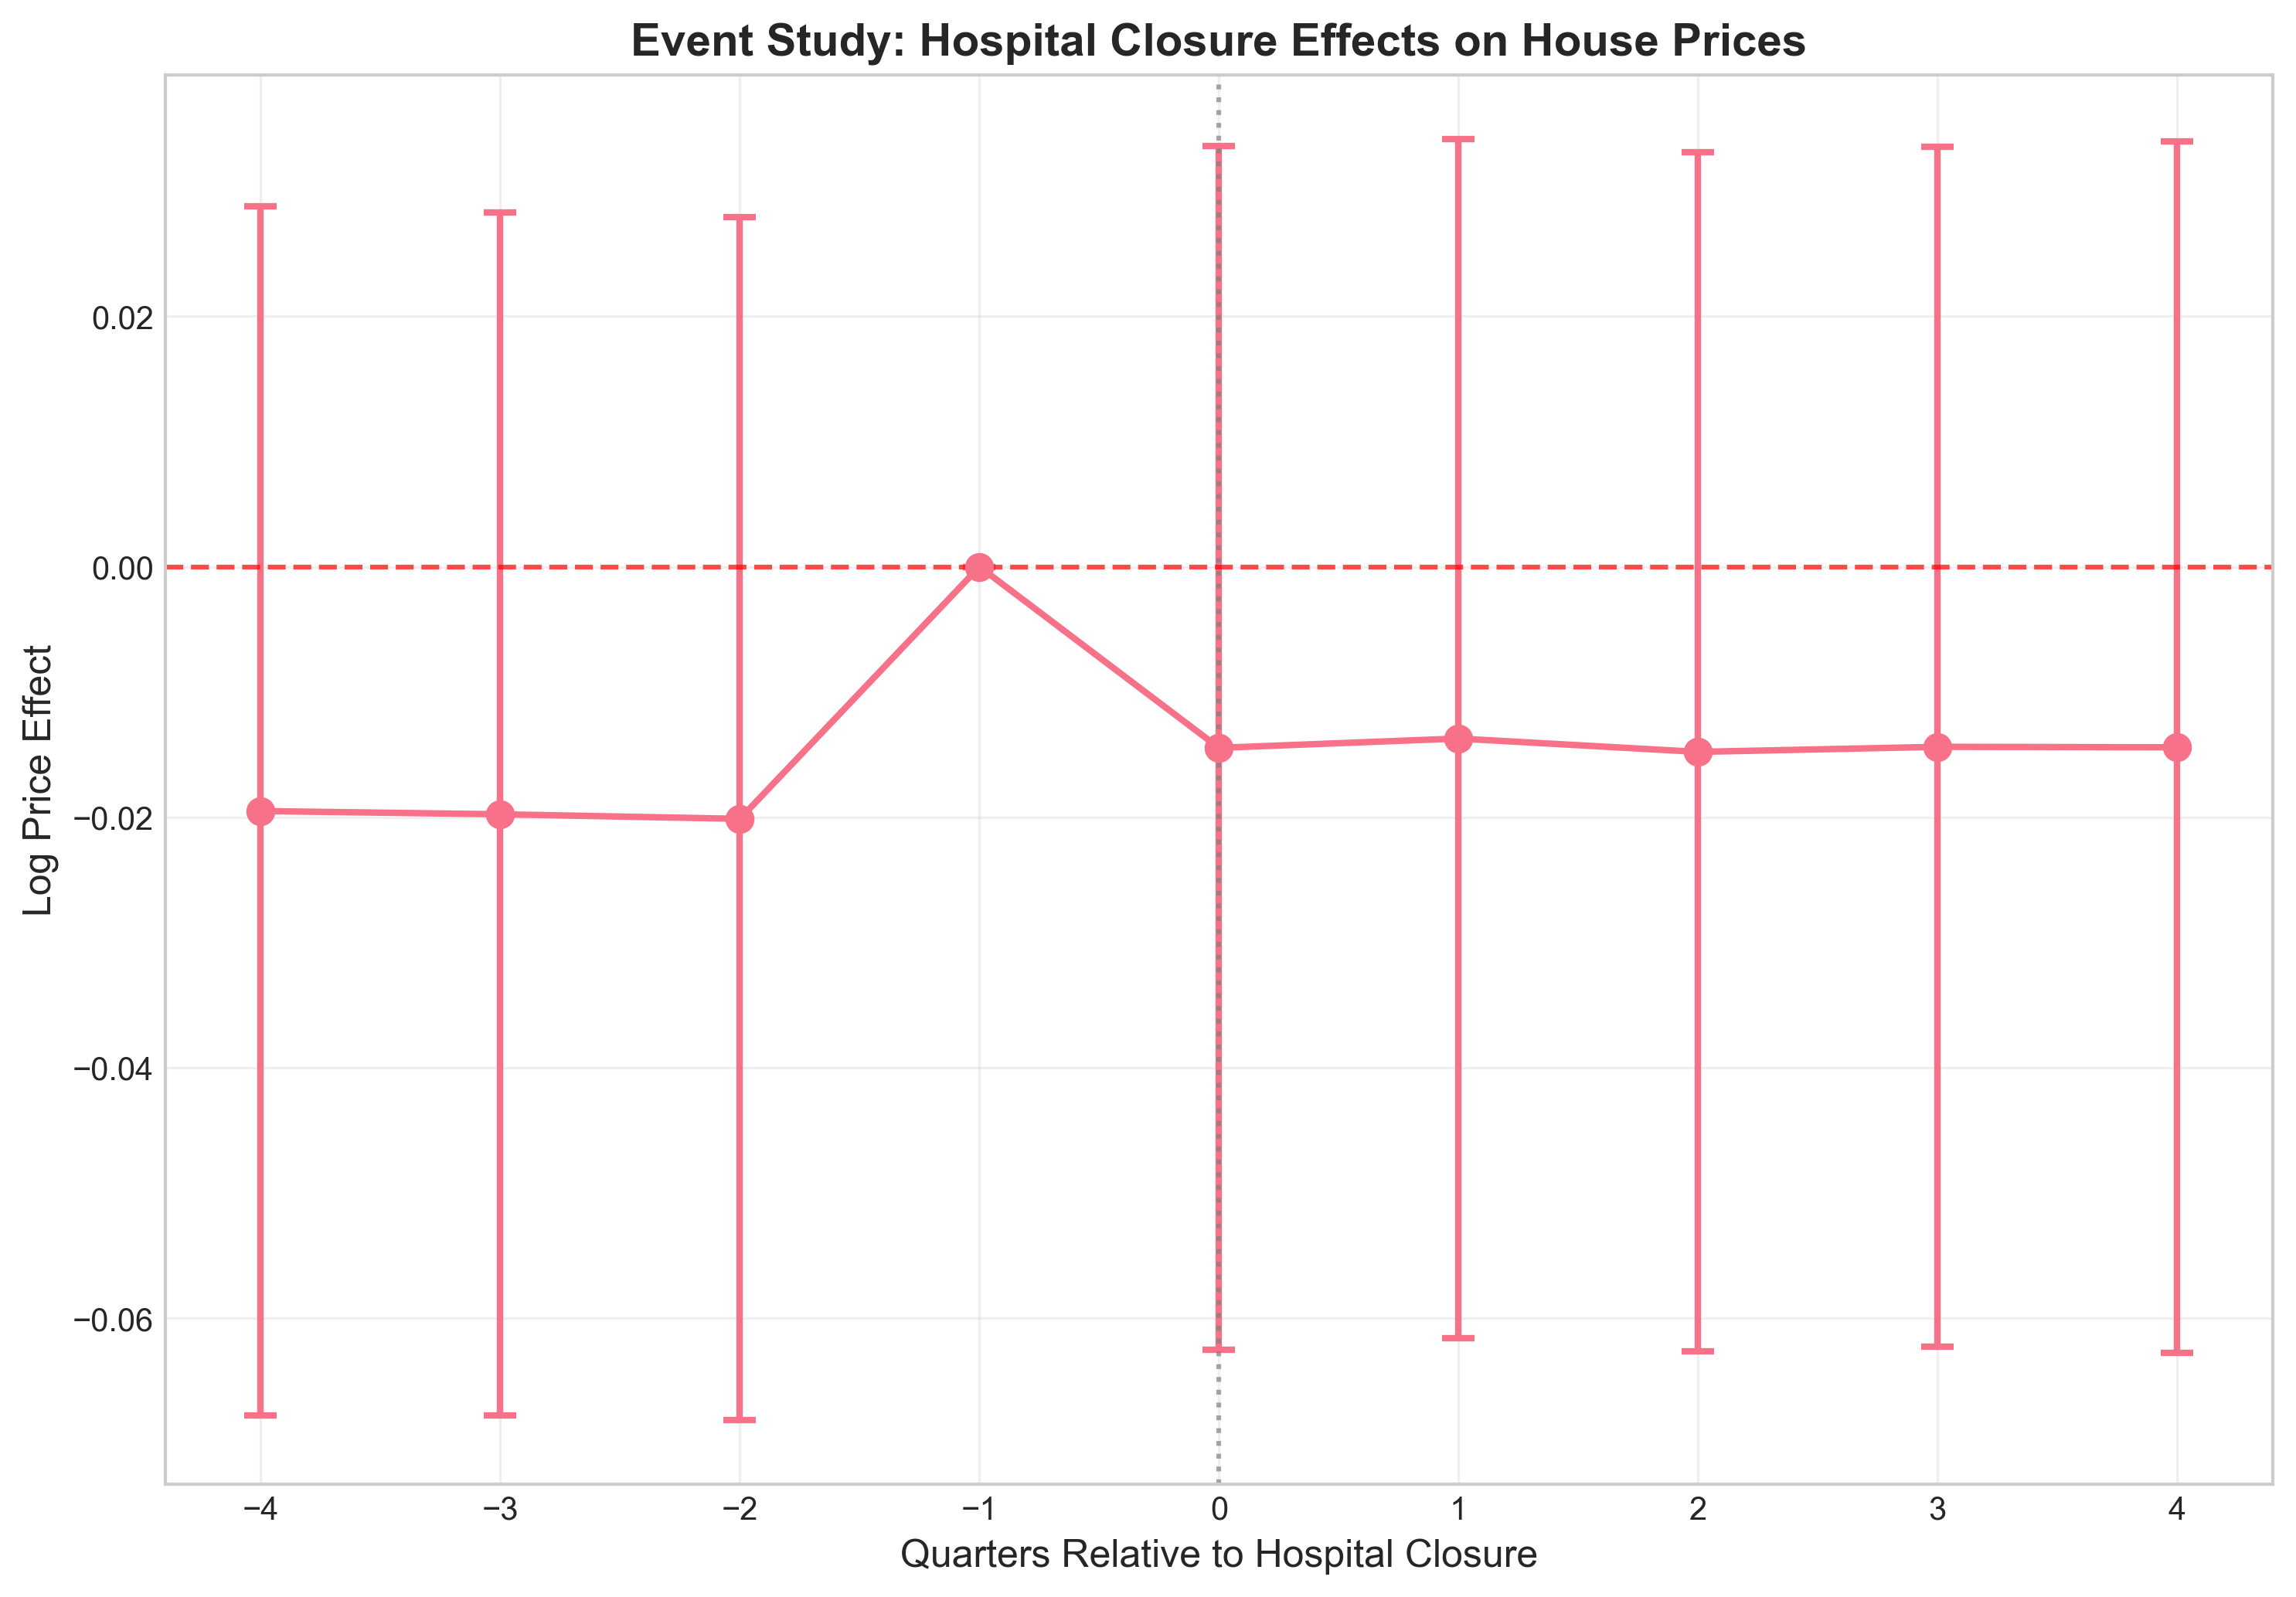
\includegraphics[width=\textwidth]{event_study_coefficients_plot.png}
\caption{Event study coefficients for the effect of rural hospital closures on house prices, using a county-quarter panel. The omitted reference period is one quarter before the closure. The shaded areas represent 95\% confidence intervals.}
\end{figure}


\section{What research questions survived these analyses?}

\begin{enumerate}
    \item Does senior migration to high healthcare amenity places drive up rents? Status: Some puzzles here in the long-differences. The existing work seems to be very reduced form, so I am optimistic on contiuing on this. 
\item How do healthcare amenities influence rent? Status: data seems to exist to answer this question, it seems worth continuing, but the objection that multiple things are happening at once in the rural-hospital closure setting is well-taken. 

\end{enumerate}

\newpage
\appendix
\section{Appendix Figures and Tables}
\begin{table}[htbp]
\caption{Summary Statistics of Variables used in Manu. / HC. analysis}
\label{tab:summary_stats}
\begin{adjustbox}{max width=\textwidth}
\begin{tabular}{lrrrrrrrr}
\toprule
 & Mean & Std. Dev. & Min & Q1 & Median & Q3 & Max & N \\
\midrule
$\Delta$ Share of Pop. 65+ (2000-10) & 0.011 & 0.014 & -0.061 & 0.002 & 0.011 & 0.018 & 0.160 & 2628 \\
Manu. Loss ($\Delta$ Share, 2000-10) & 0.085 & 0.103 & -0.323 & 0.023 & 0.059 & 0.113 & 0.658 & 2628 \\
$\Delta$ HC Share (2000-2010) & 0.021 & 0.069 & -0.448 & 0.009 & 0.033 & 0.054 & 0.246 & 2628 \\
HC Share (2000) & 0.143 & 0.059 & 0.009 & 0.101 & 0.137 & 0.174 & 0.545 & 2628 \\
Share of Pop. 65+ (2000) & 0.144 & 0.039 & 0.023 & 0.119 & 0.142 & 0.166 & 0.347 & 2628 \\
 Total Pop. (2000, thousands) & 104.631 & 314.327 & 1.902 & 16.349 & 32.845 & 75.792 & 9519.338 & 2628 \\
\bottomrule
\end{tabular}
\end{adjustbox}
\end{table}

\begin{table}[htbp]
\centering
\caption{Regression Results: Net Migration Rate 65+ (2010-2020)}
\label{tab:netmig_regression}
\begin{tabular}{lcc}
\hline\hline
 & Coefficient & Std. Error \\
\hline
Baseline Pop. 65+ Share (2010) & 3.966$^{***}$ & (0.317) \\
Median HH Income (\$000s) & 3.813$^{***}$ & (0.323) \\
Rural Indicator & -3.004$^{***}$ & (0.276) \\
Region: West & 2.932$^{***}$ & (0.314) \\
Region: South & 2.755$^{***}$ & (0.255) \\
Median House Value (\$0000s) & -2.515$^{***}$ & (0.359) \\
Hispanic Pop. Share & -2.251$^{***}$ & (0.235) \\
Log Total Population & 2.100$^{***}$ & (0.355) \\
Pop. 55-64 Share (2010) & -1.710$^{***}$ & (0.313) \\
Natural Amenities Scale & 1.433$^{***}$ & (0.324) \\
Coastal County & -1.100$^{***}$ & (0.212) \\
Seasonal Housing Share & -0.692$^{***}$ & (0.199) \\
State Income Tax Rate & -0.405$^{*}$ & (0.211) \\
Metro Indicator & 0.147 & (0.277) \\
College Enrollment Share & -0.146 & (0.398) \\
Private School Market Share & 0.090 & (0.404) \\
Intercept & 4.035$^{***}$ & (0.186) \\
\hline
Observations & 3105 & \\
$R^2$ & 0.224 & \\
\hline\hline
\multicolumn{3}{l}{\footnotesize $^{*}p<0.1$; $^{**}p<0.05$; $^{***}p<0.01$} \\
\end{tabular}
\end{table}
\begin{table}[htbp]
\caption{Top 10 Counties by Increase in Elderly Population Count (2000-2010)}
\label{tab:top10_elderly_count_increase}
\begin{tabular}{clrrrr}
\toprule
 & County & Pop. (2000) & Pop. (2010) & Pop. 65+ (2000) & $\Delta$ Count 65+ \\
\midrule
1 & Los Angeles County, California & 9,519,338 & 9,818,605 & 926,673 & 139,026 \\
2 & Maricopa County, Arizona & 3,072,149 & 3,817,117 & 358,979 & 103,662 \\
3 & Harris County, Texas & 3,400,578 & 4,092,459 & 252,895 & 80,592 \\
4 & Clark County, Nevada & 1,375,765 & 1,951,269 & 146,899 & 73,546 \\
5 & Orange County, California & 2,846,289 & 3,010,232 & 280,763 & 68,914 \\
6 & Riverside County, California & 1,545,387 & 2,189,641 & 195,963 & 62,622 \\
7 & Tarrant County, Texas & 1,446,219 & 1,809,034 & 120,585 & 40,800 \\
8 & San Diego County, California & 2,813,833 & 3,095,313 & 313,750 & 37,675 \\
9 & Santa Clara County, California & 1,682,585 & 1,781,642 & 160,527 & 36,417 \\
10 & San Bernardino County, California & 1,709,434 & 2,035,210 & 146,459 & 34,889 \\
\bottomrule
\\
\multicolumn{6}{l}{\footnotesize Note: Limited to counties with population $\geq$ 100,000 in 2000.} \\
\end{tabular}
\end{table}

\begin{table}[htbp]
\caption{Bottom 10 Counties by Change in Elderly Population Share (2000-2010)}
\label{tab:bottom10_elderly_change}
\begin{tabular}{clrrrr}
\toprule
 & County & Pop. (2000) & Pop. (2010) & Pct. 65+ (2000, \%) & $\Delta$ Share 65+ (pp) \\
\midrule
1 & Lee County, Florida & 440,888 & 618,754 & 25.43 & -1.98 \\
2 & Indian River County, Florida & 112,947 & 138,028 & 29.19 & -2.02 \\
3 & Benton County, Arkansas & 153,406 & 221,339 & 14.32 & -2.13 \\
4 & Richmond city, Virginia & 197,790 & 204,214 & 13.21 & -2.13 \\
5 & Lake County, Florida & 210,528 & 297,052 & 26.41 & -2.23 \\
6 & Pinal County, Arizona & 179,727 & 375,770 & 16.23 & -2.37 \\
7 & St. Louis city, Missouri & 348,189 & 319,294 & 13.74 & -2.72 \\
8 & St. Lucie County, Florida & 192,695 & 277,789 & 22.71 & -2.77 \\
9 & Hernando County, Florida & 130,802 & 172,778 & 30.85 & -5.08 \\
10 & Pasco County, Florida & 344,765 & 464,697 & 26.80 & -6.09 \\
\bottomrule
\\
\multicolumn{6}{l}{\footnotesize Note: Limited to counties with population $\geq$ 100,000 in 2000.} \\
\end{tabular}
\end{table}

\begin{table}[htbp]
\caption{Bottom 10 Counties by Change in Elderly Population Count (2000-2010)}
\label{tab:bottom10_elderly_count_change}
\begin{tabular}{clrrrr}
\toprule
 & County & Pop. (2000) & Pop. (2010) & Pop. 65+ (2000) & $\Delta$ Count 65+ \\
\midrule
1 & Philadelphia County, Pennsylvania & 1,517,550 & 1,526,006 & 213,722 & -28,413 \\
2 & Allegheny County, Pennsylvania & 1,281,666 & 1,223,348 & 228,416 & -23,357 \\
3 & Orleans Parish, Louisiana & 484,674 & 343,829 & 56,653 & -19,014 \\
4 & Cuyahoga County, Ohio & 1,393,978 & 1,280,122 & 217,161 & -18,620 \\
5 & Wayne County, Michigan & 2,061,162 & 1,820,584 & 248,982 & -18,279 \\
6 & Pinellas County, Florida & 921,482 & 916,542 & 207,563 & -13,464 \\
7 & Baltimore city, Maryland & 651,154 & 620,961 & 85,921 & -13,109 \\
8 & St. Louis city, Missouri & 348,189 & 319,294 & 47,842 & -12,667 \\
9 & Milwaukee County, Wisconsin & 940,164 & 947,735 & 121,684 & -12,551 \\
10 & Broward County, Florida & 1,623,018 & 1,748,066 & 261,109 & -11,685 \\
\bottomrule
\\
\multicolumn{6}{l}{\footnotesize Note: Limited to counties with population $\geq$ 100,000 in 2000.} \\
\end{tabular}
\end{table}



\begin{figure}[htbp]
    \centering
    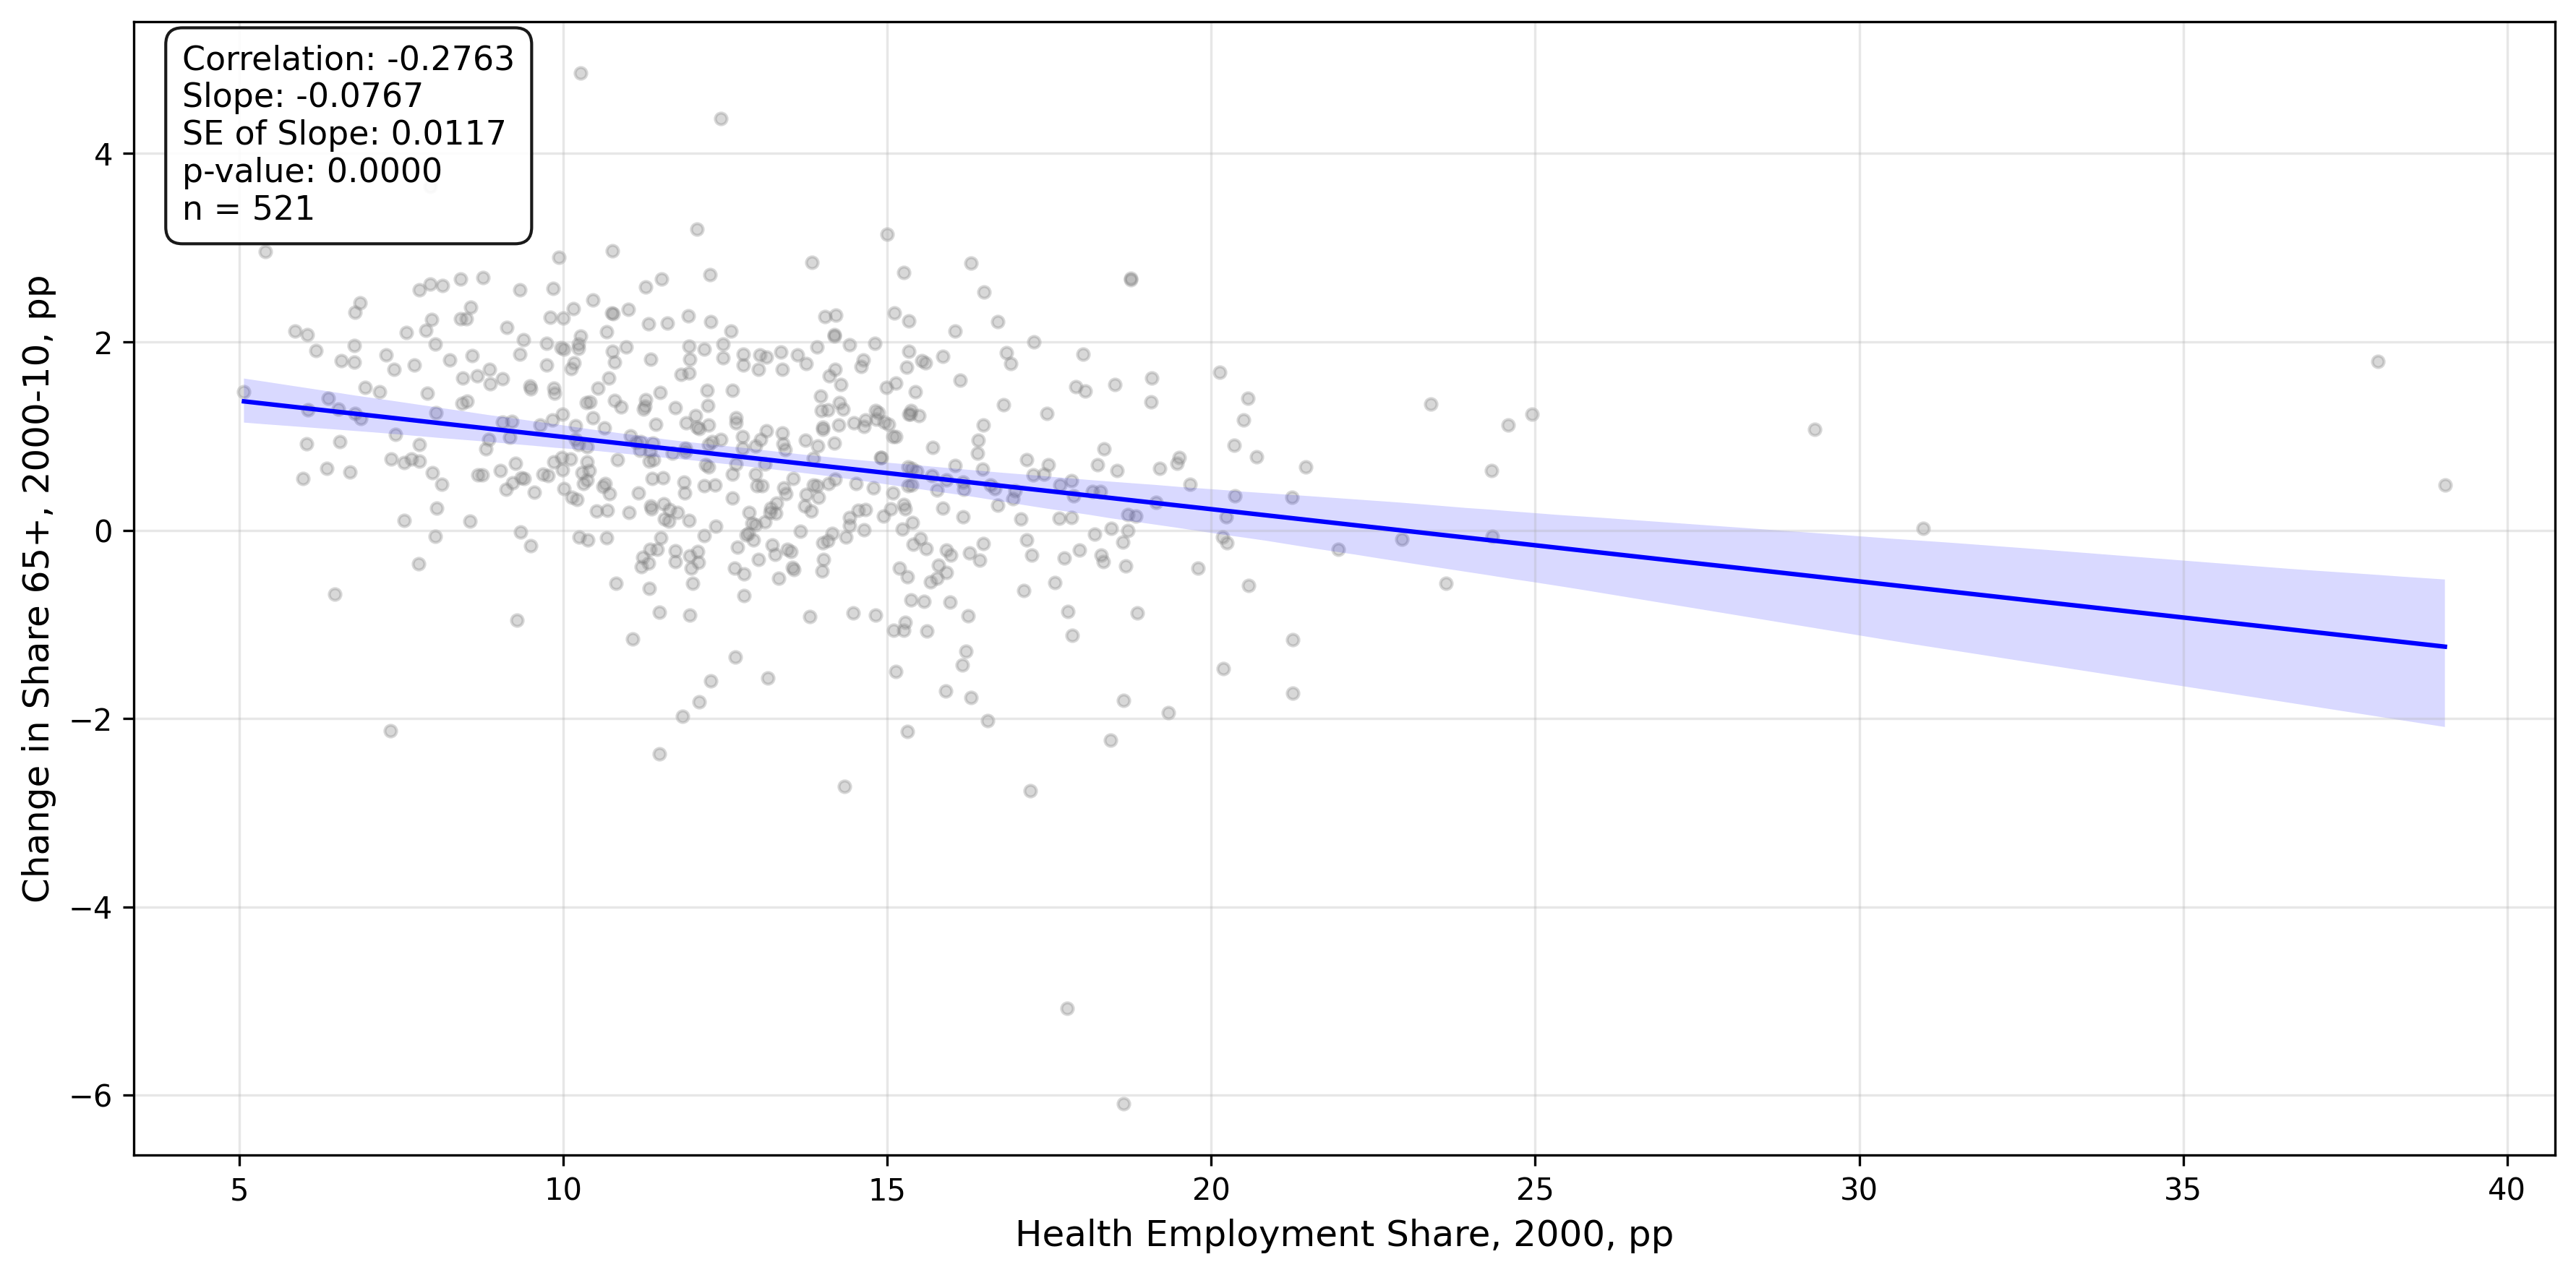
\includegraphics[width=0.96\textwidth]{share_change_65.png}
    \caption{Correlation of healthcare employment share (2000) and change in elderly population share, (2000-2010), restricted to counties with 2000 population of 100K or more. Counties are observations.   }
    \label{fig:aggregate_health_change}
\end{figure}



\begin{figure}[htbp]
    \centering
    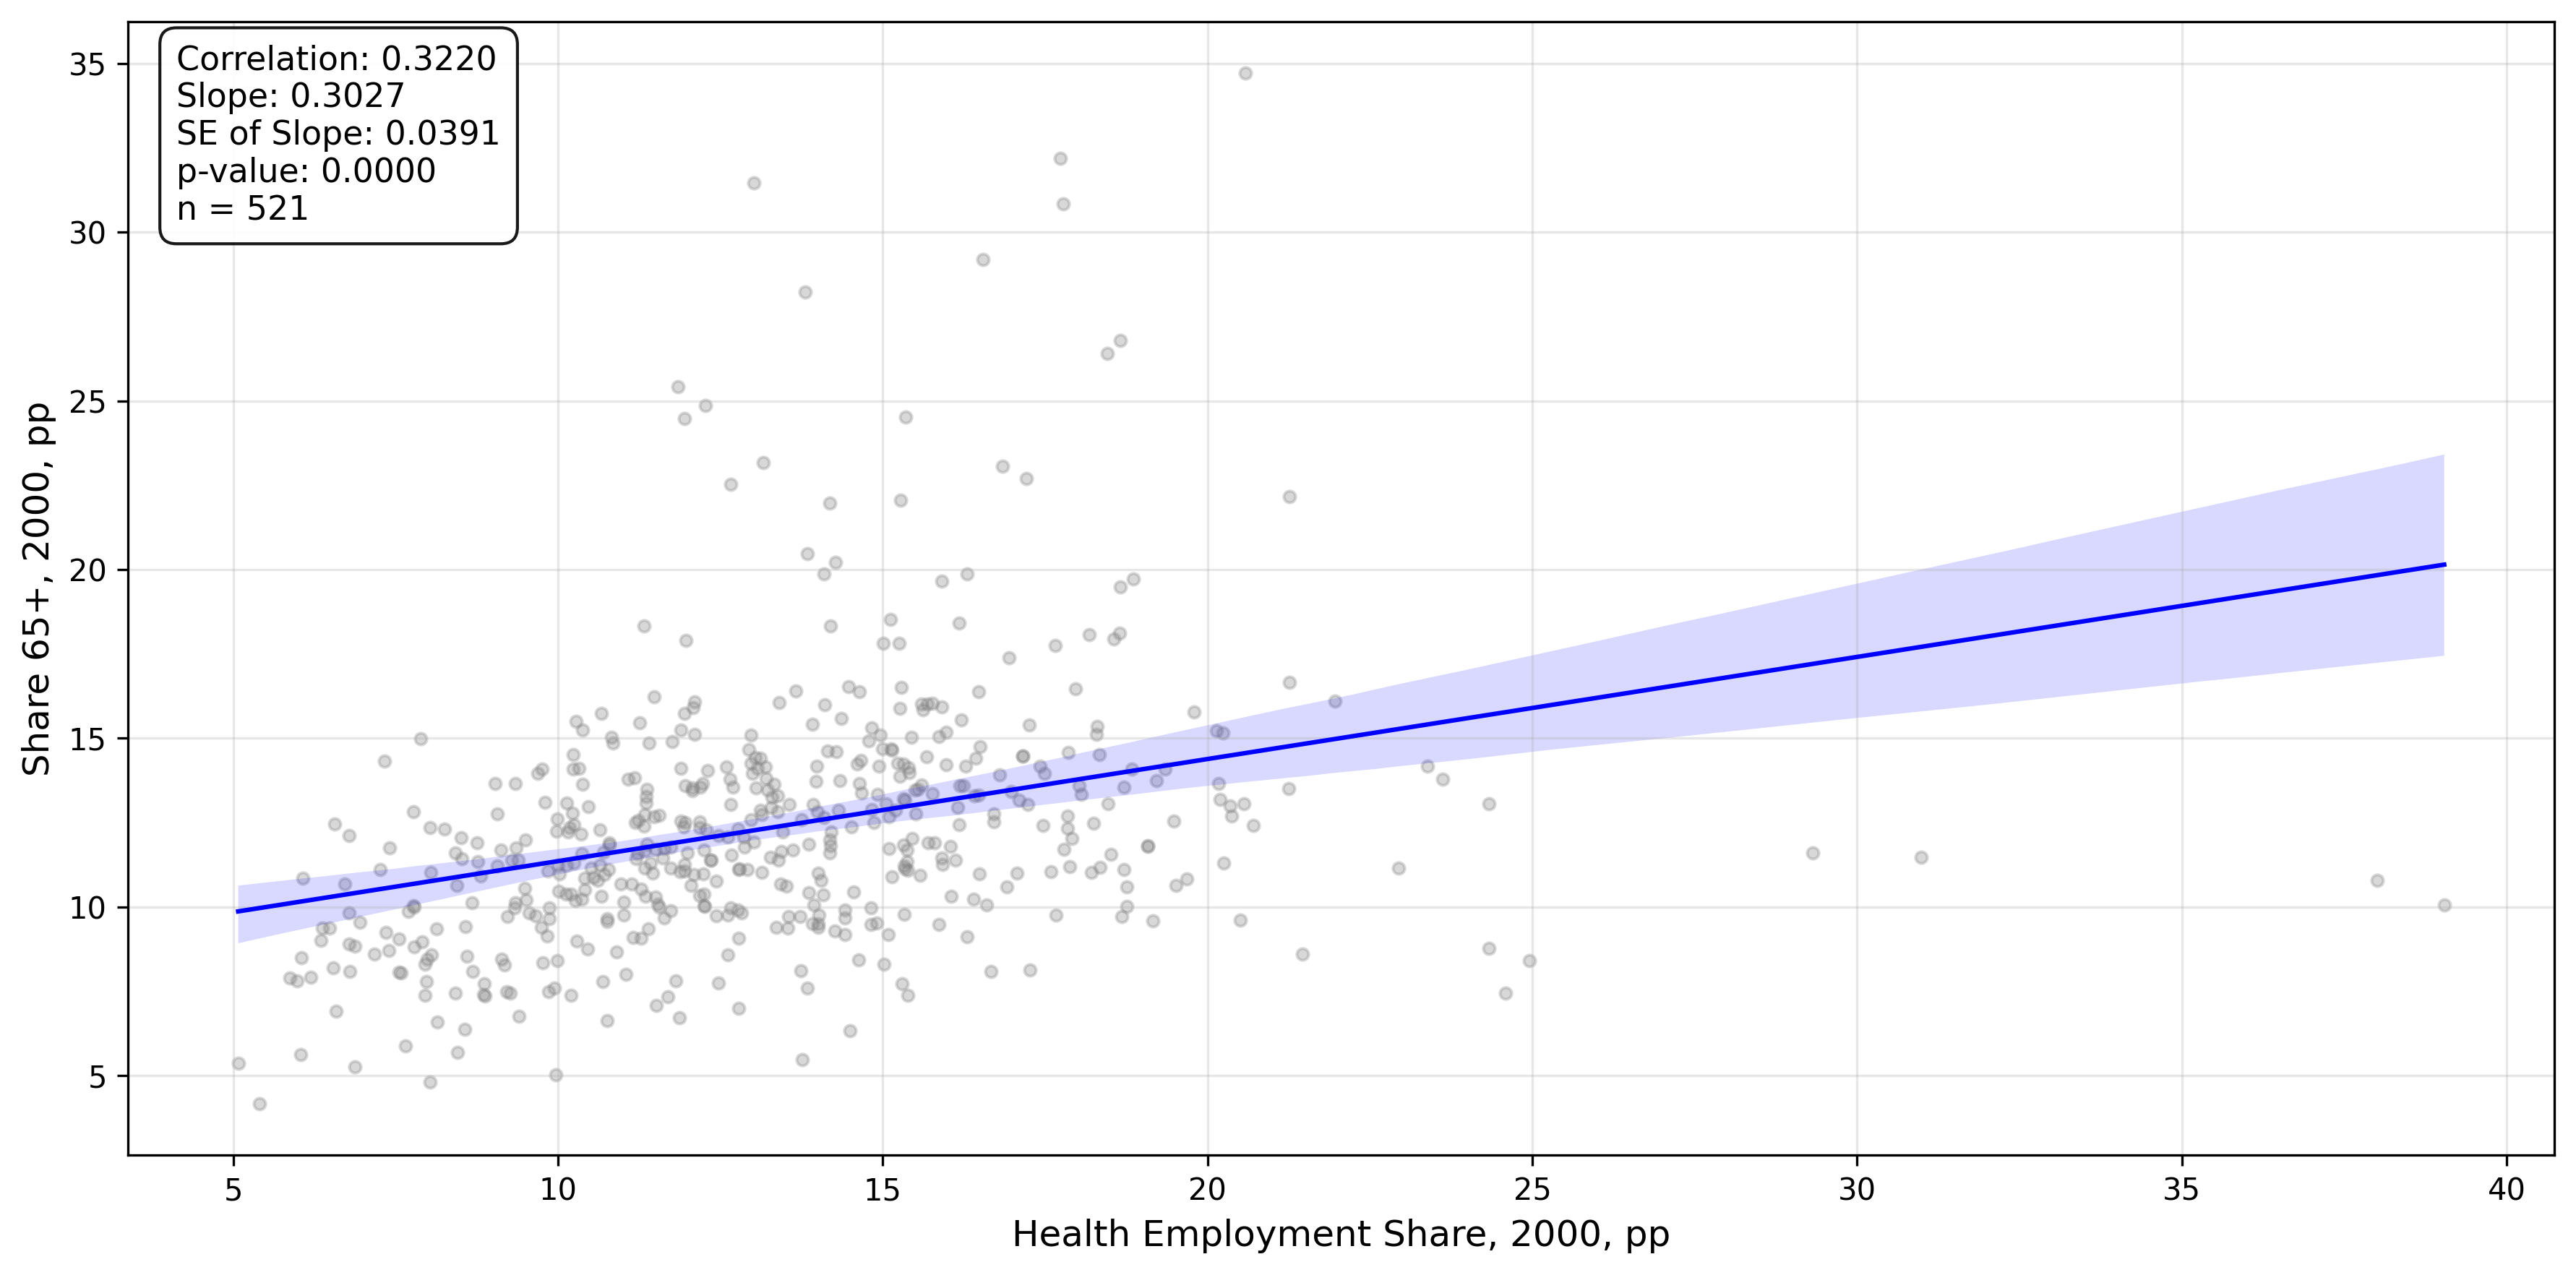
\includegraphics[width=0.96\textwidth]{HealthOld2000.png}
    \caption{Correlation of healthcare employment share and elderly population share, 2000, restricted to counties with 2000 population of 100K or more. Counties are observations.   }
    \label{fig:HealthOld2000}
    \end{figure}

    \begin{figure}[htbp]
        \centering
        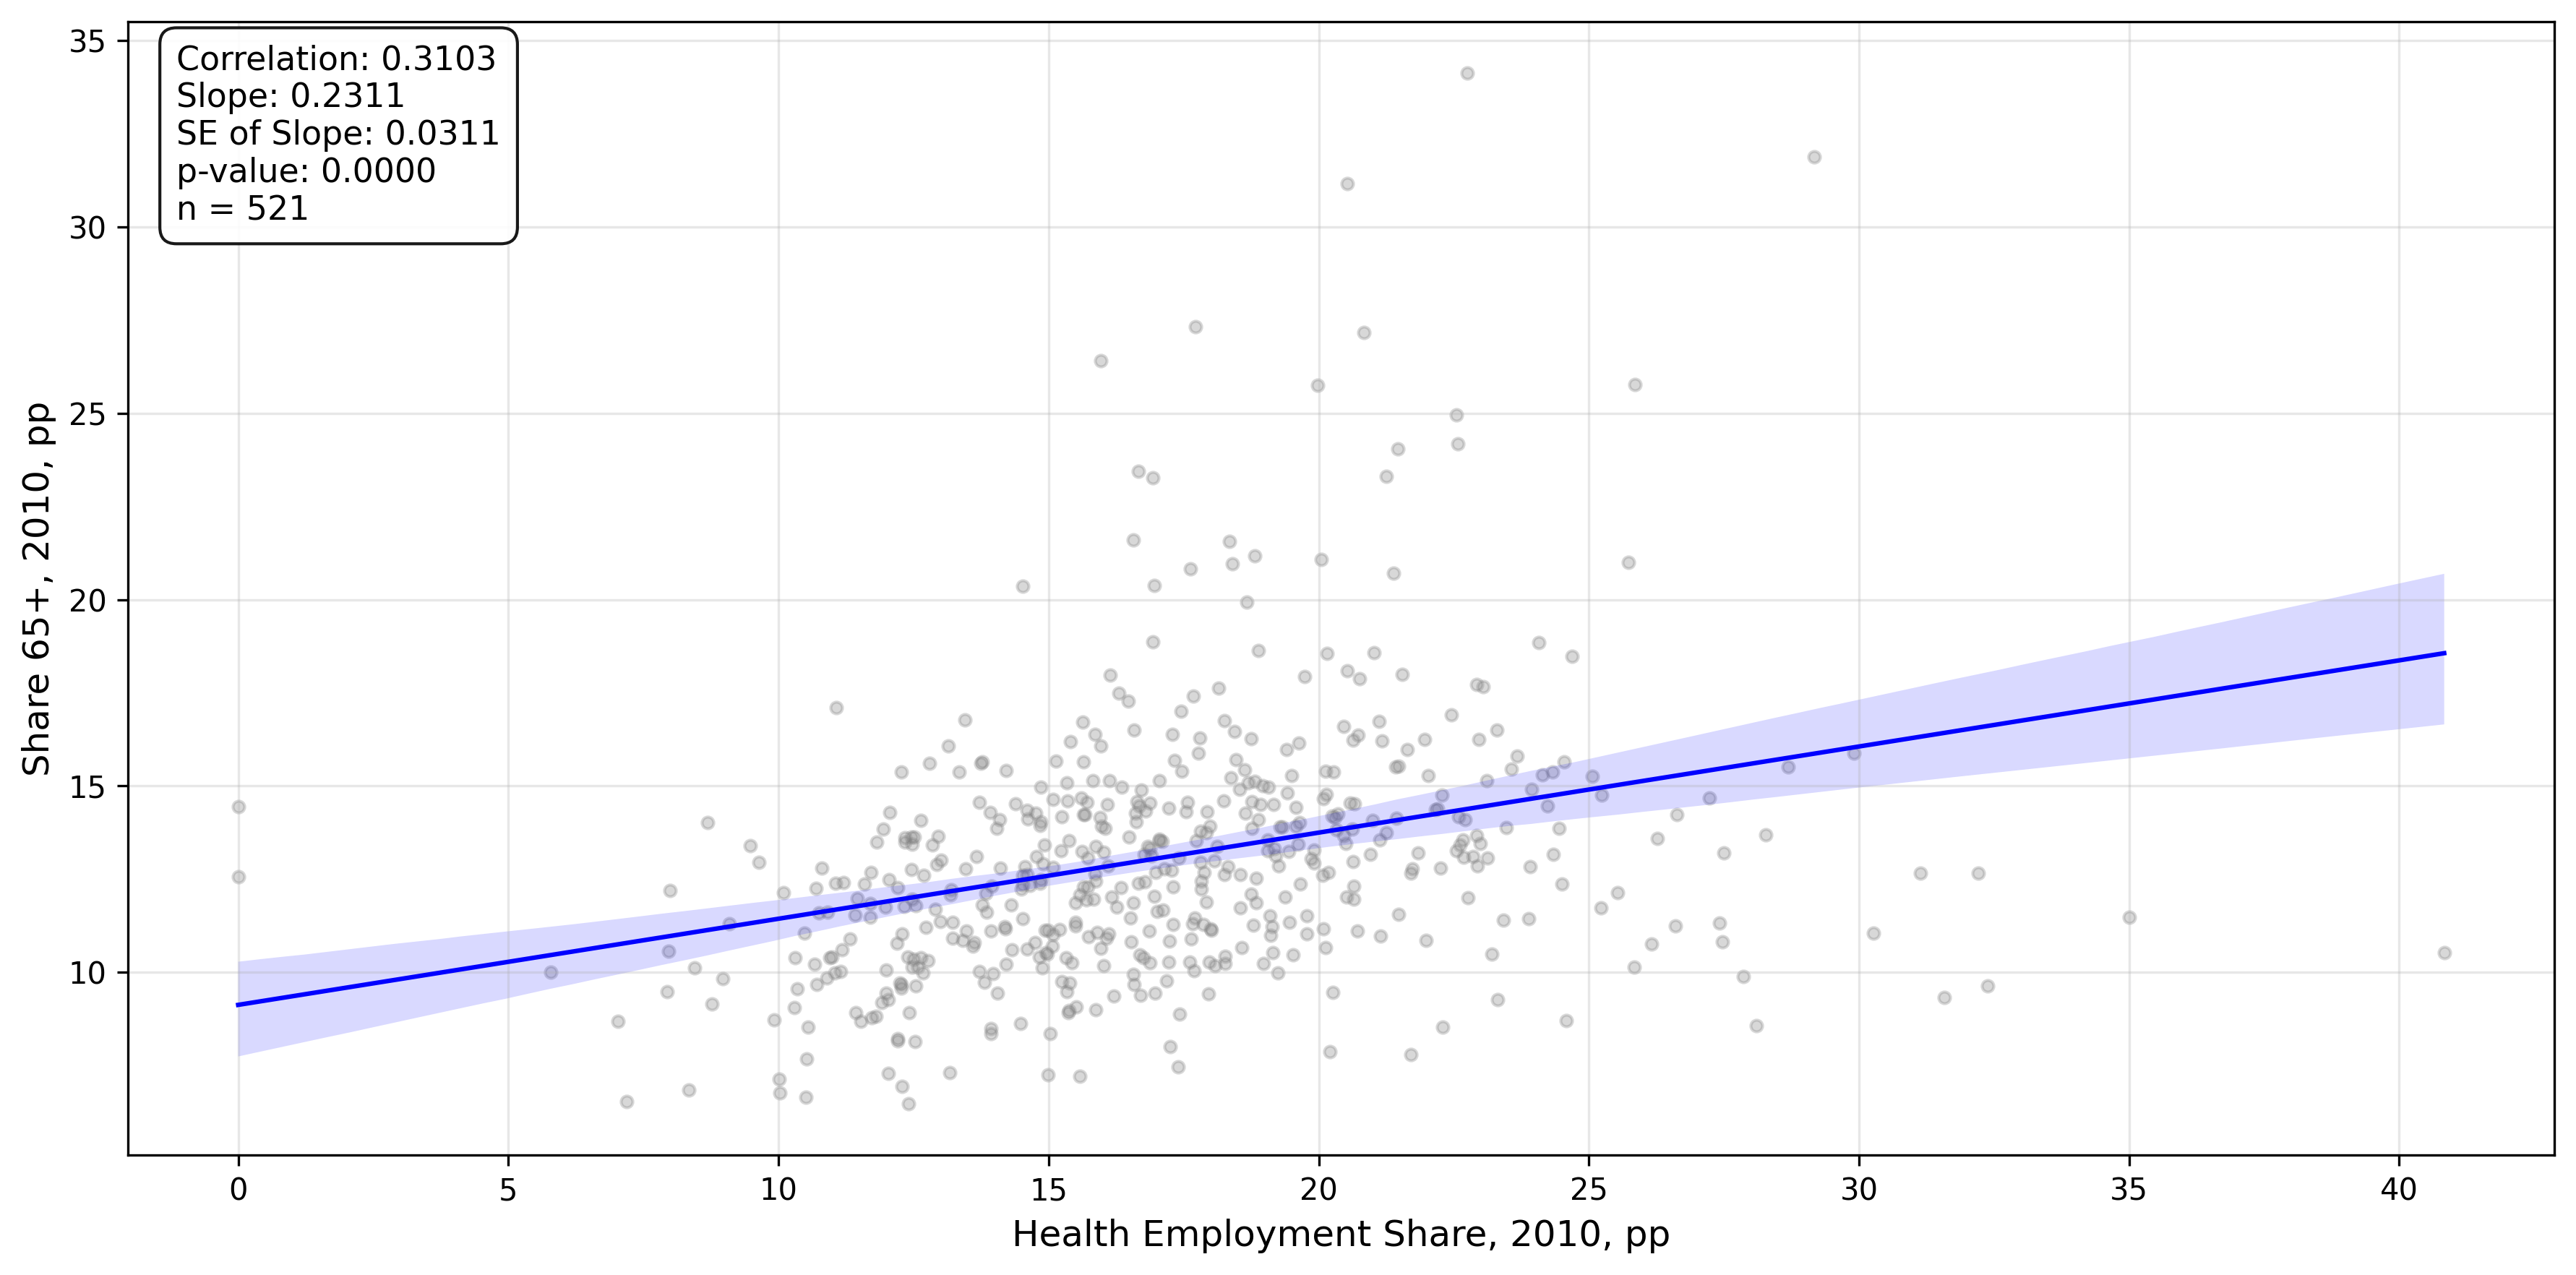
\includegraphics[width=0.96\textwidth]{HealthOld2010.png}
        \caption{Correlation of healthcare employment share and elderly population share, 2010, restricted to counties with 2000 population of 100K or more. Counties are observations.   }
        \label{fig:HealthOld2010}
    \end{figure}

    \begin{figure}[htbp]
        \centering
        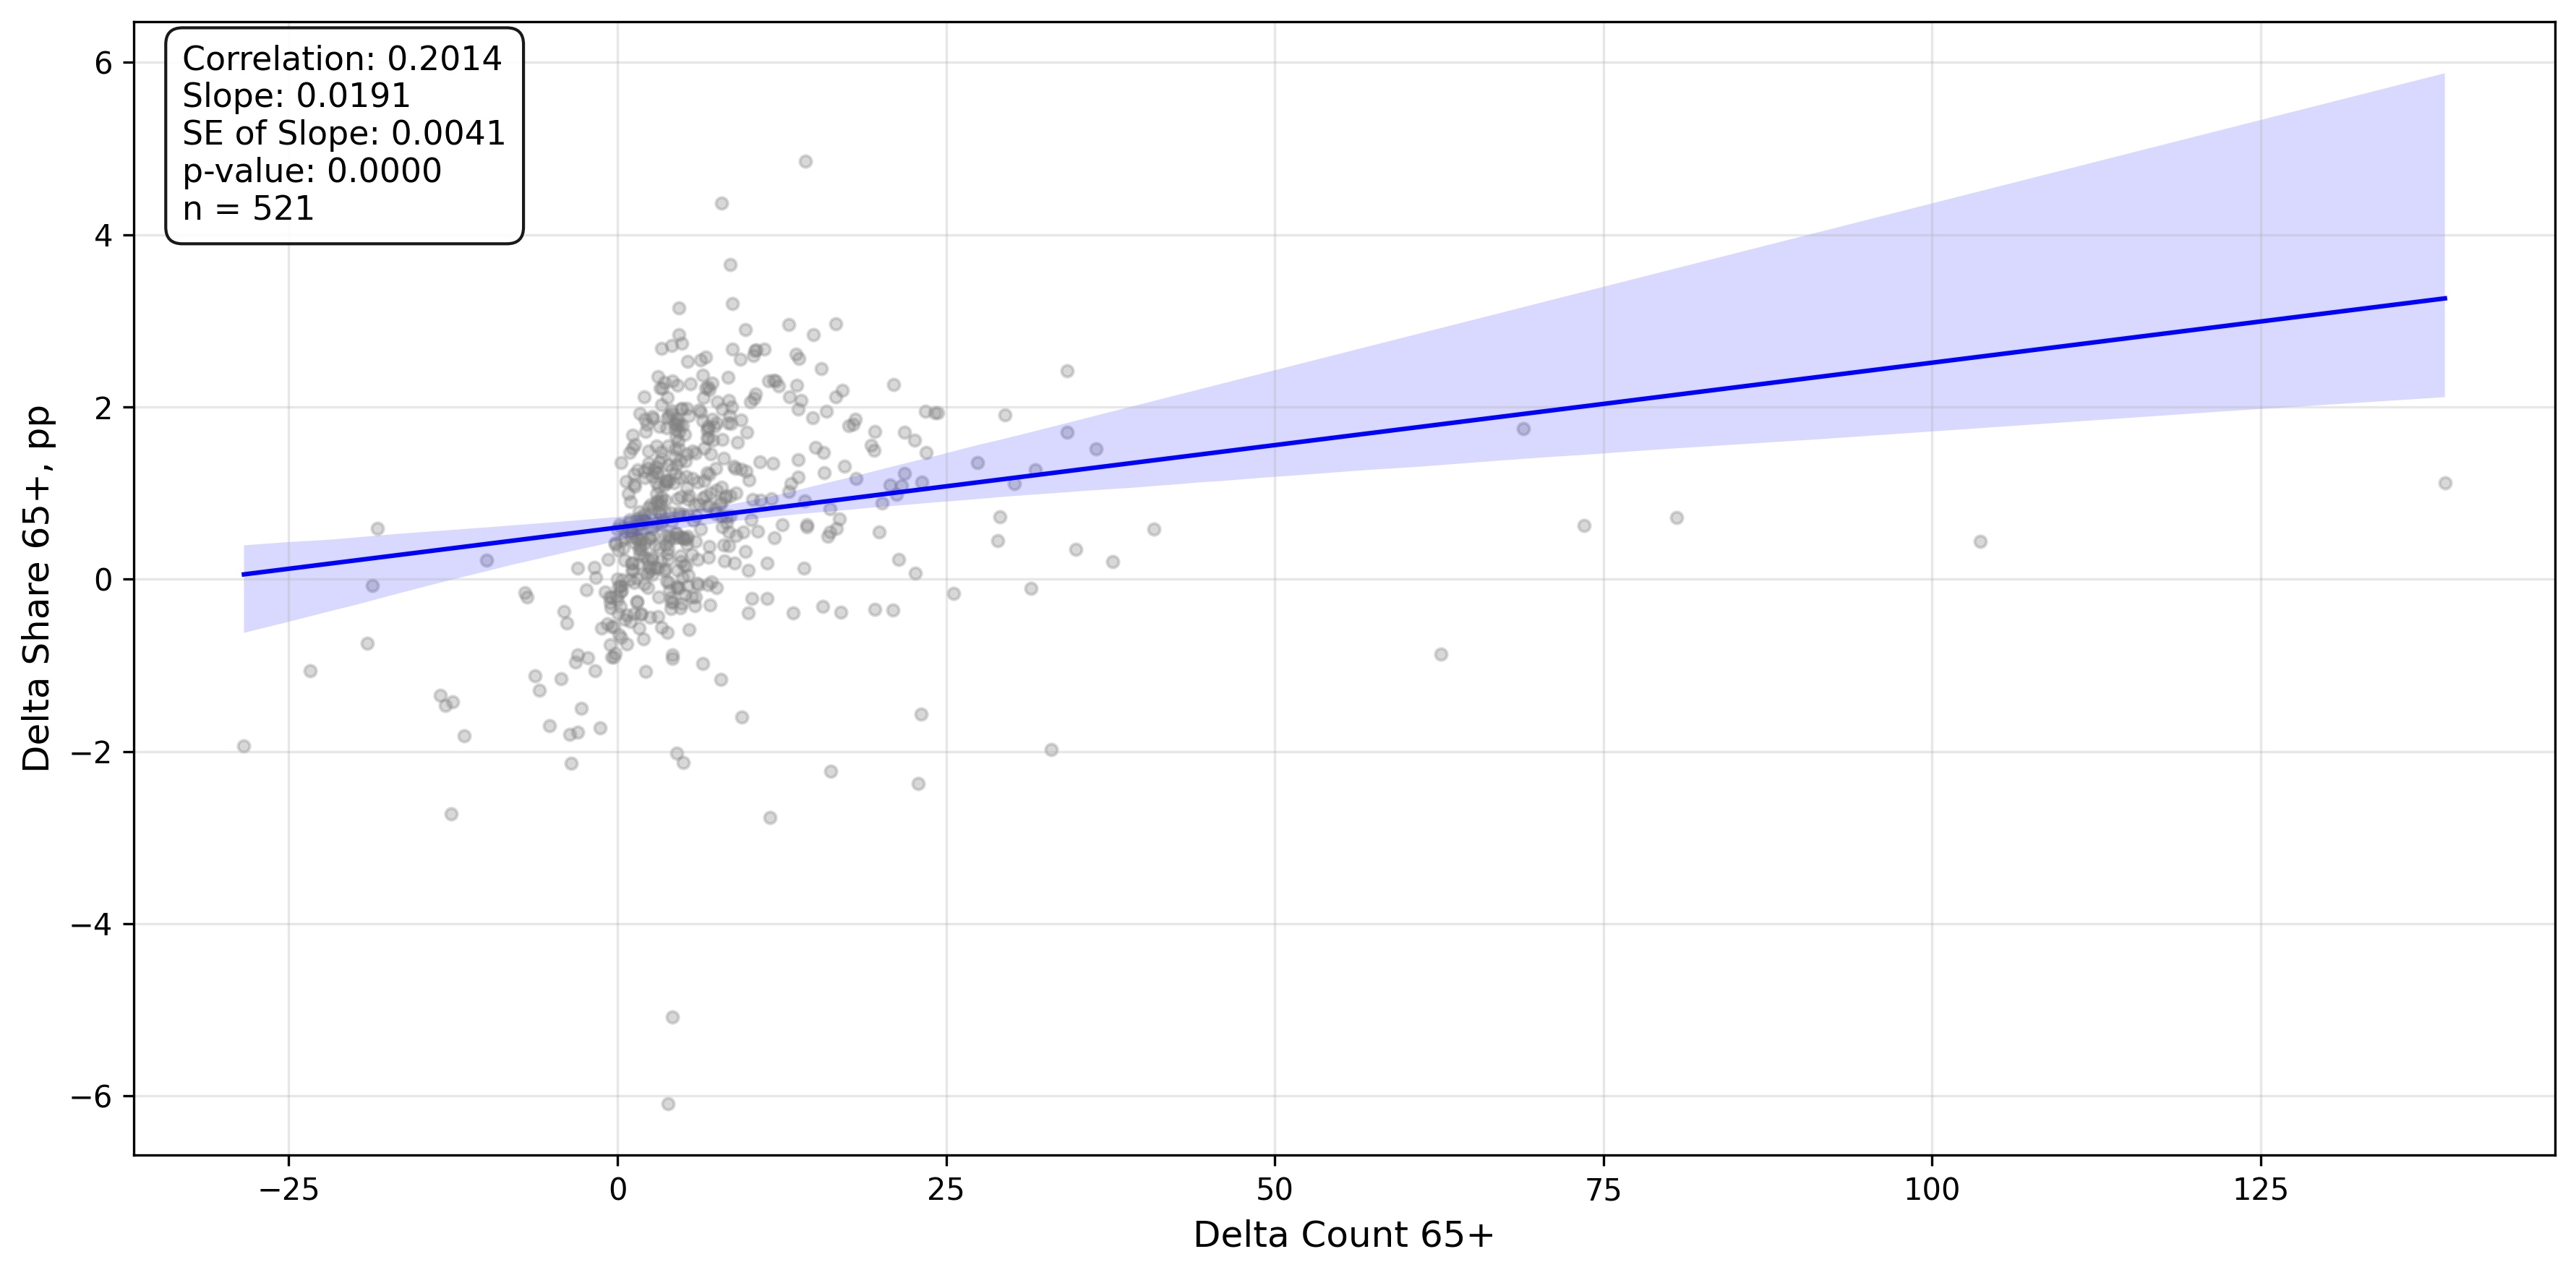
\includegraphics[width=0.96\textwidth]{delta_count_vs_share_analysis.png}
        \caption{Correlation of changes in counts and shares of the 65+ population, restricted to counties with 2000 population of 100K or more. Counties are observations.  }
        \end{figure}




        \newpage

    \section{Appendix on Rural Hospital Closures}
\begin{figure}
    \centering
    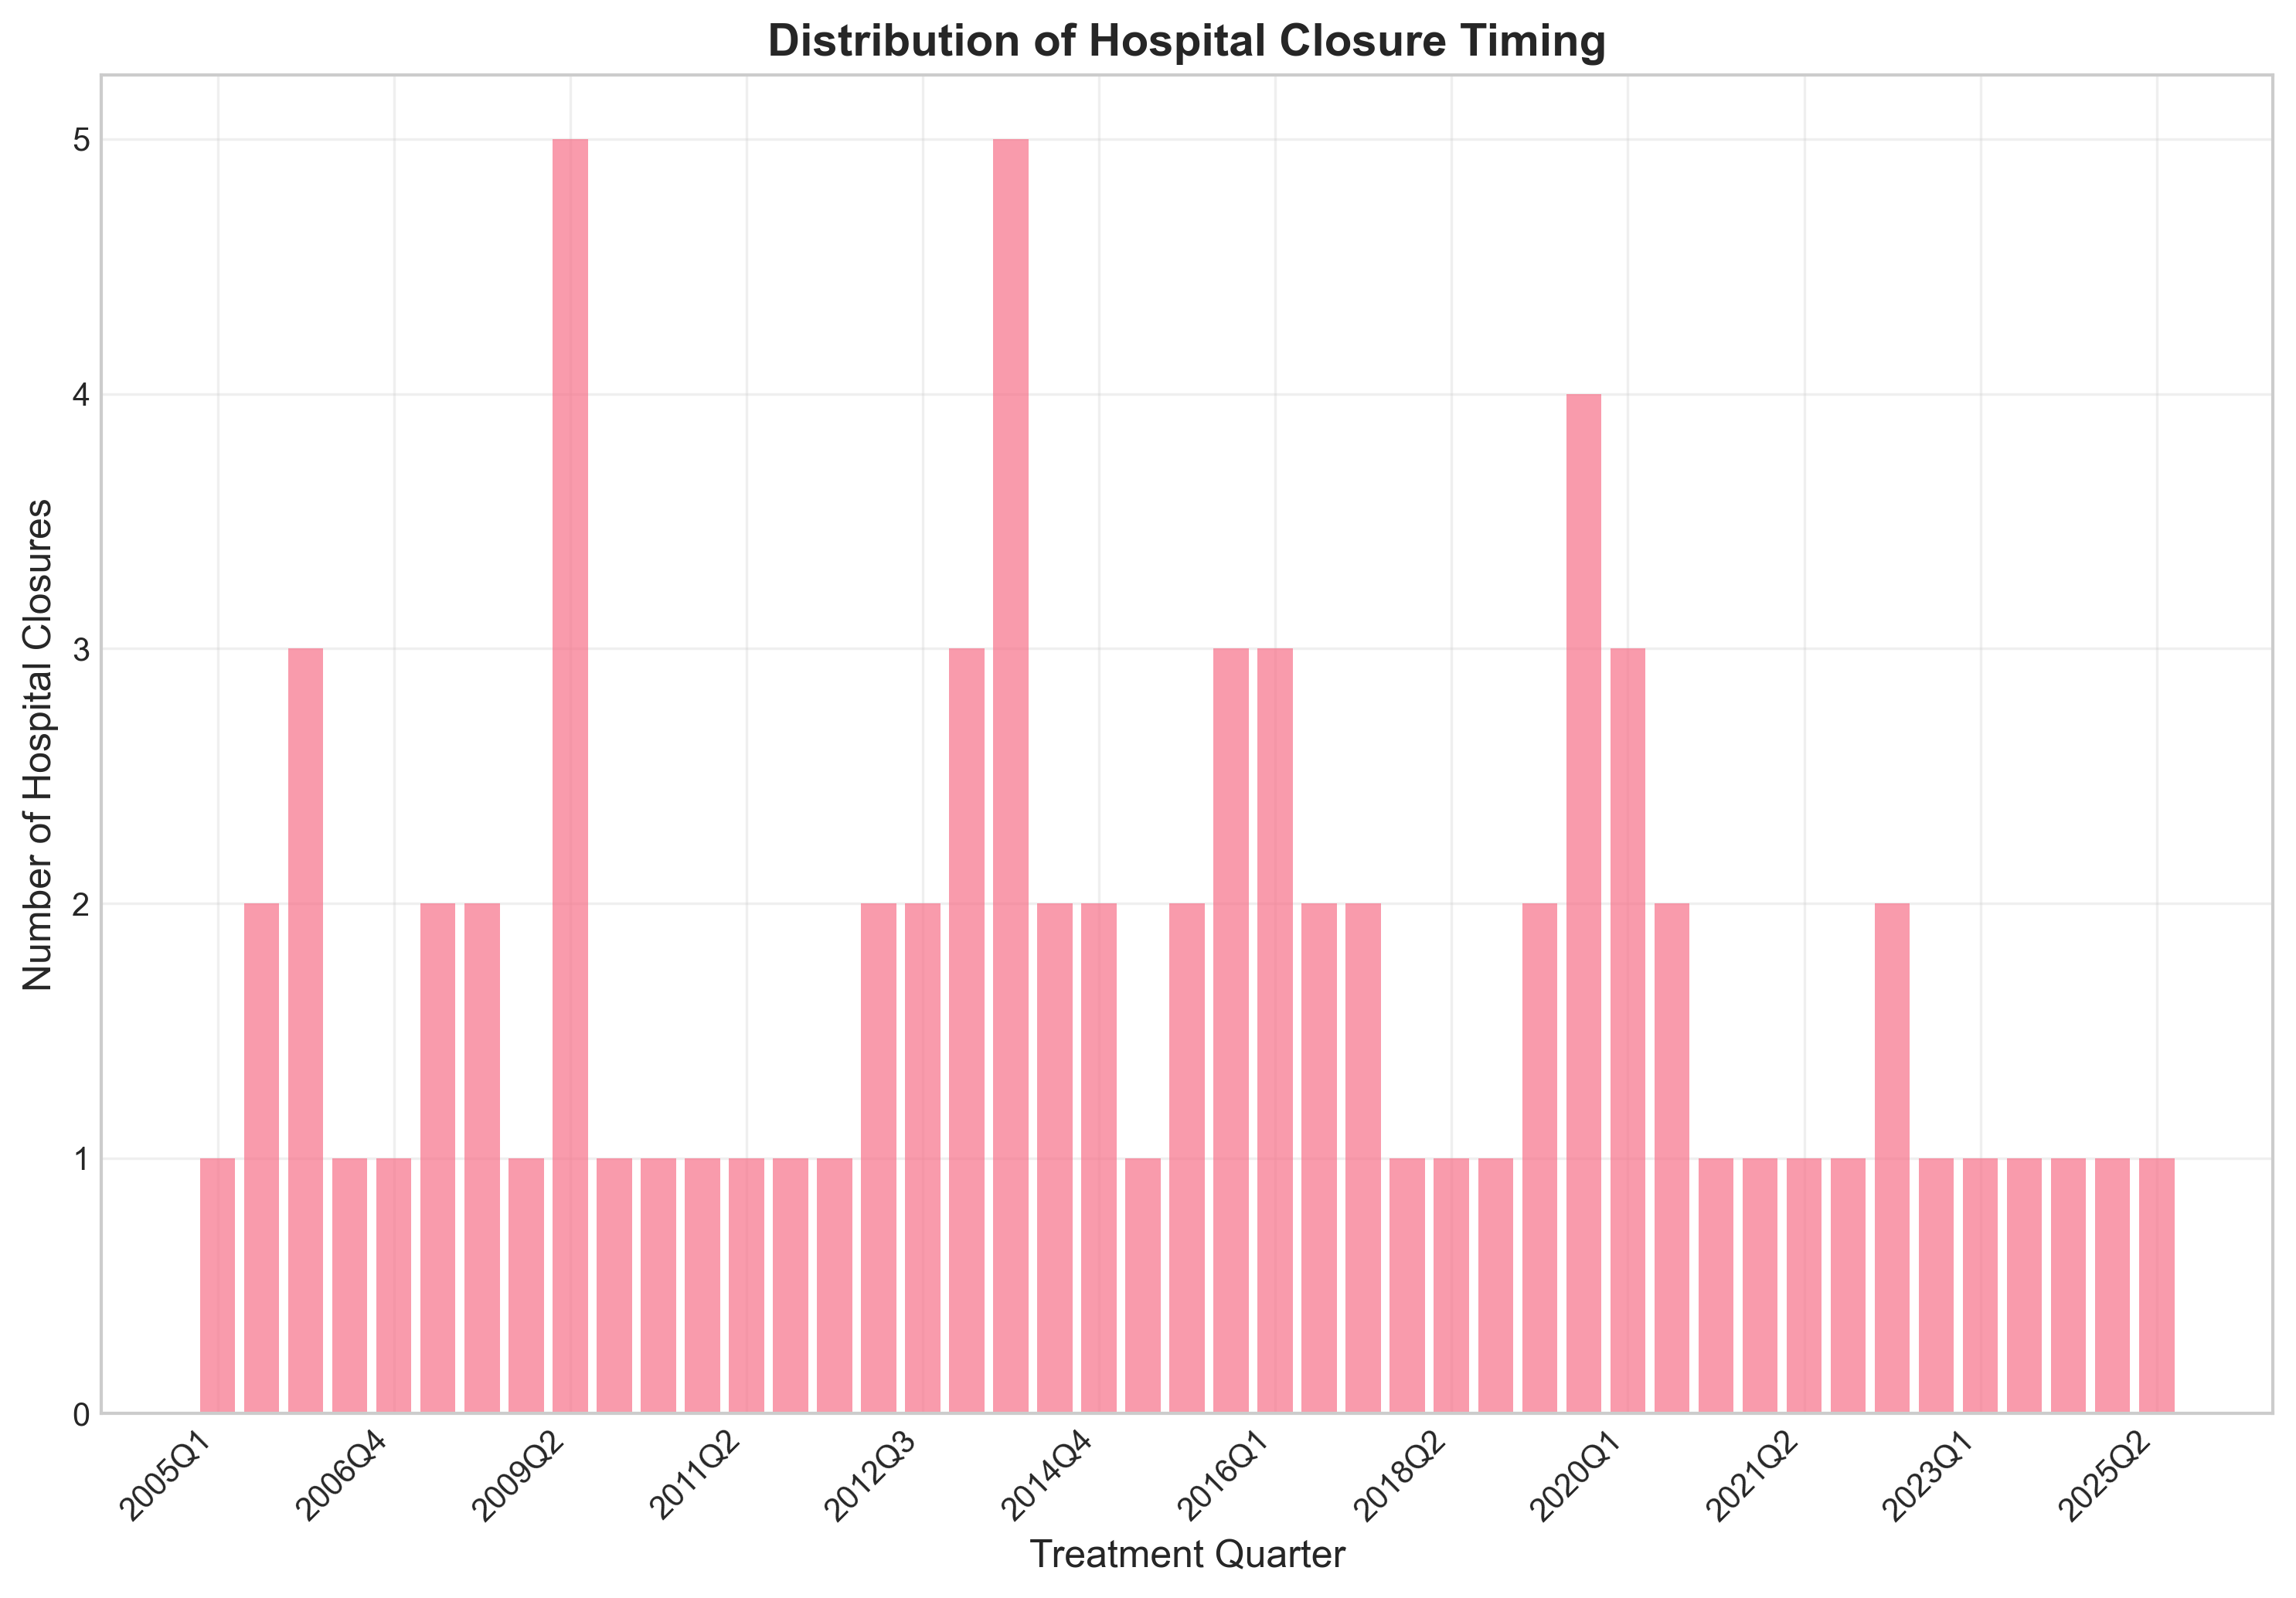
\includegraphics[width=0.96\textwidth]{treatment_timing_distribution_plot.png}
    \caption{Dates of rural hospital closures, 2005-2025. }
    \label{fig:closure_dates}
\end{figure}


\begin{figure}
    \centering
    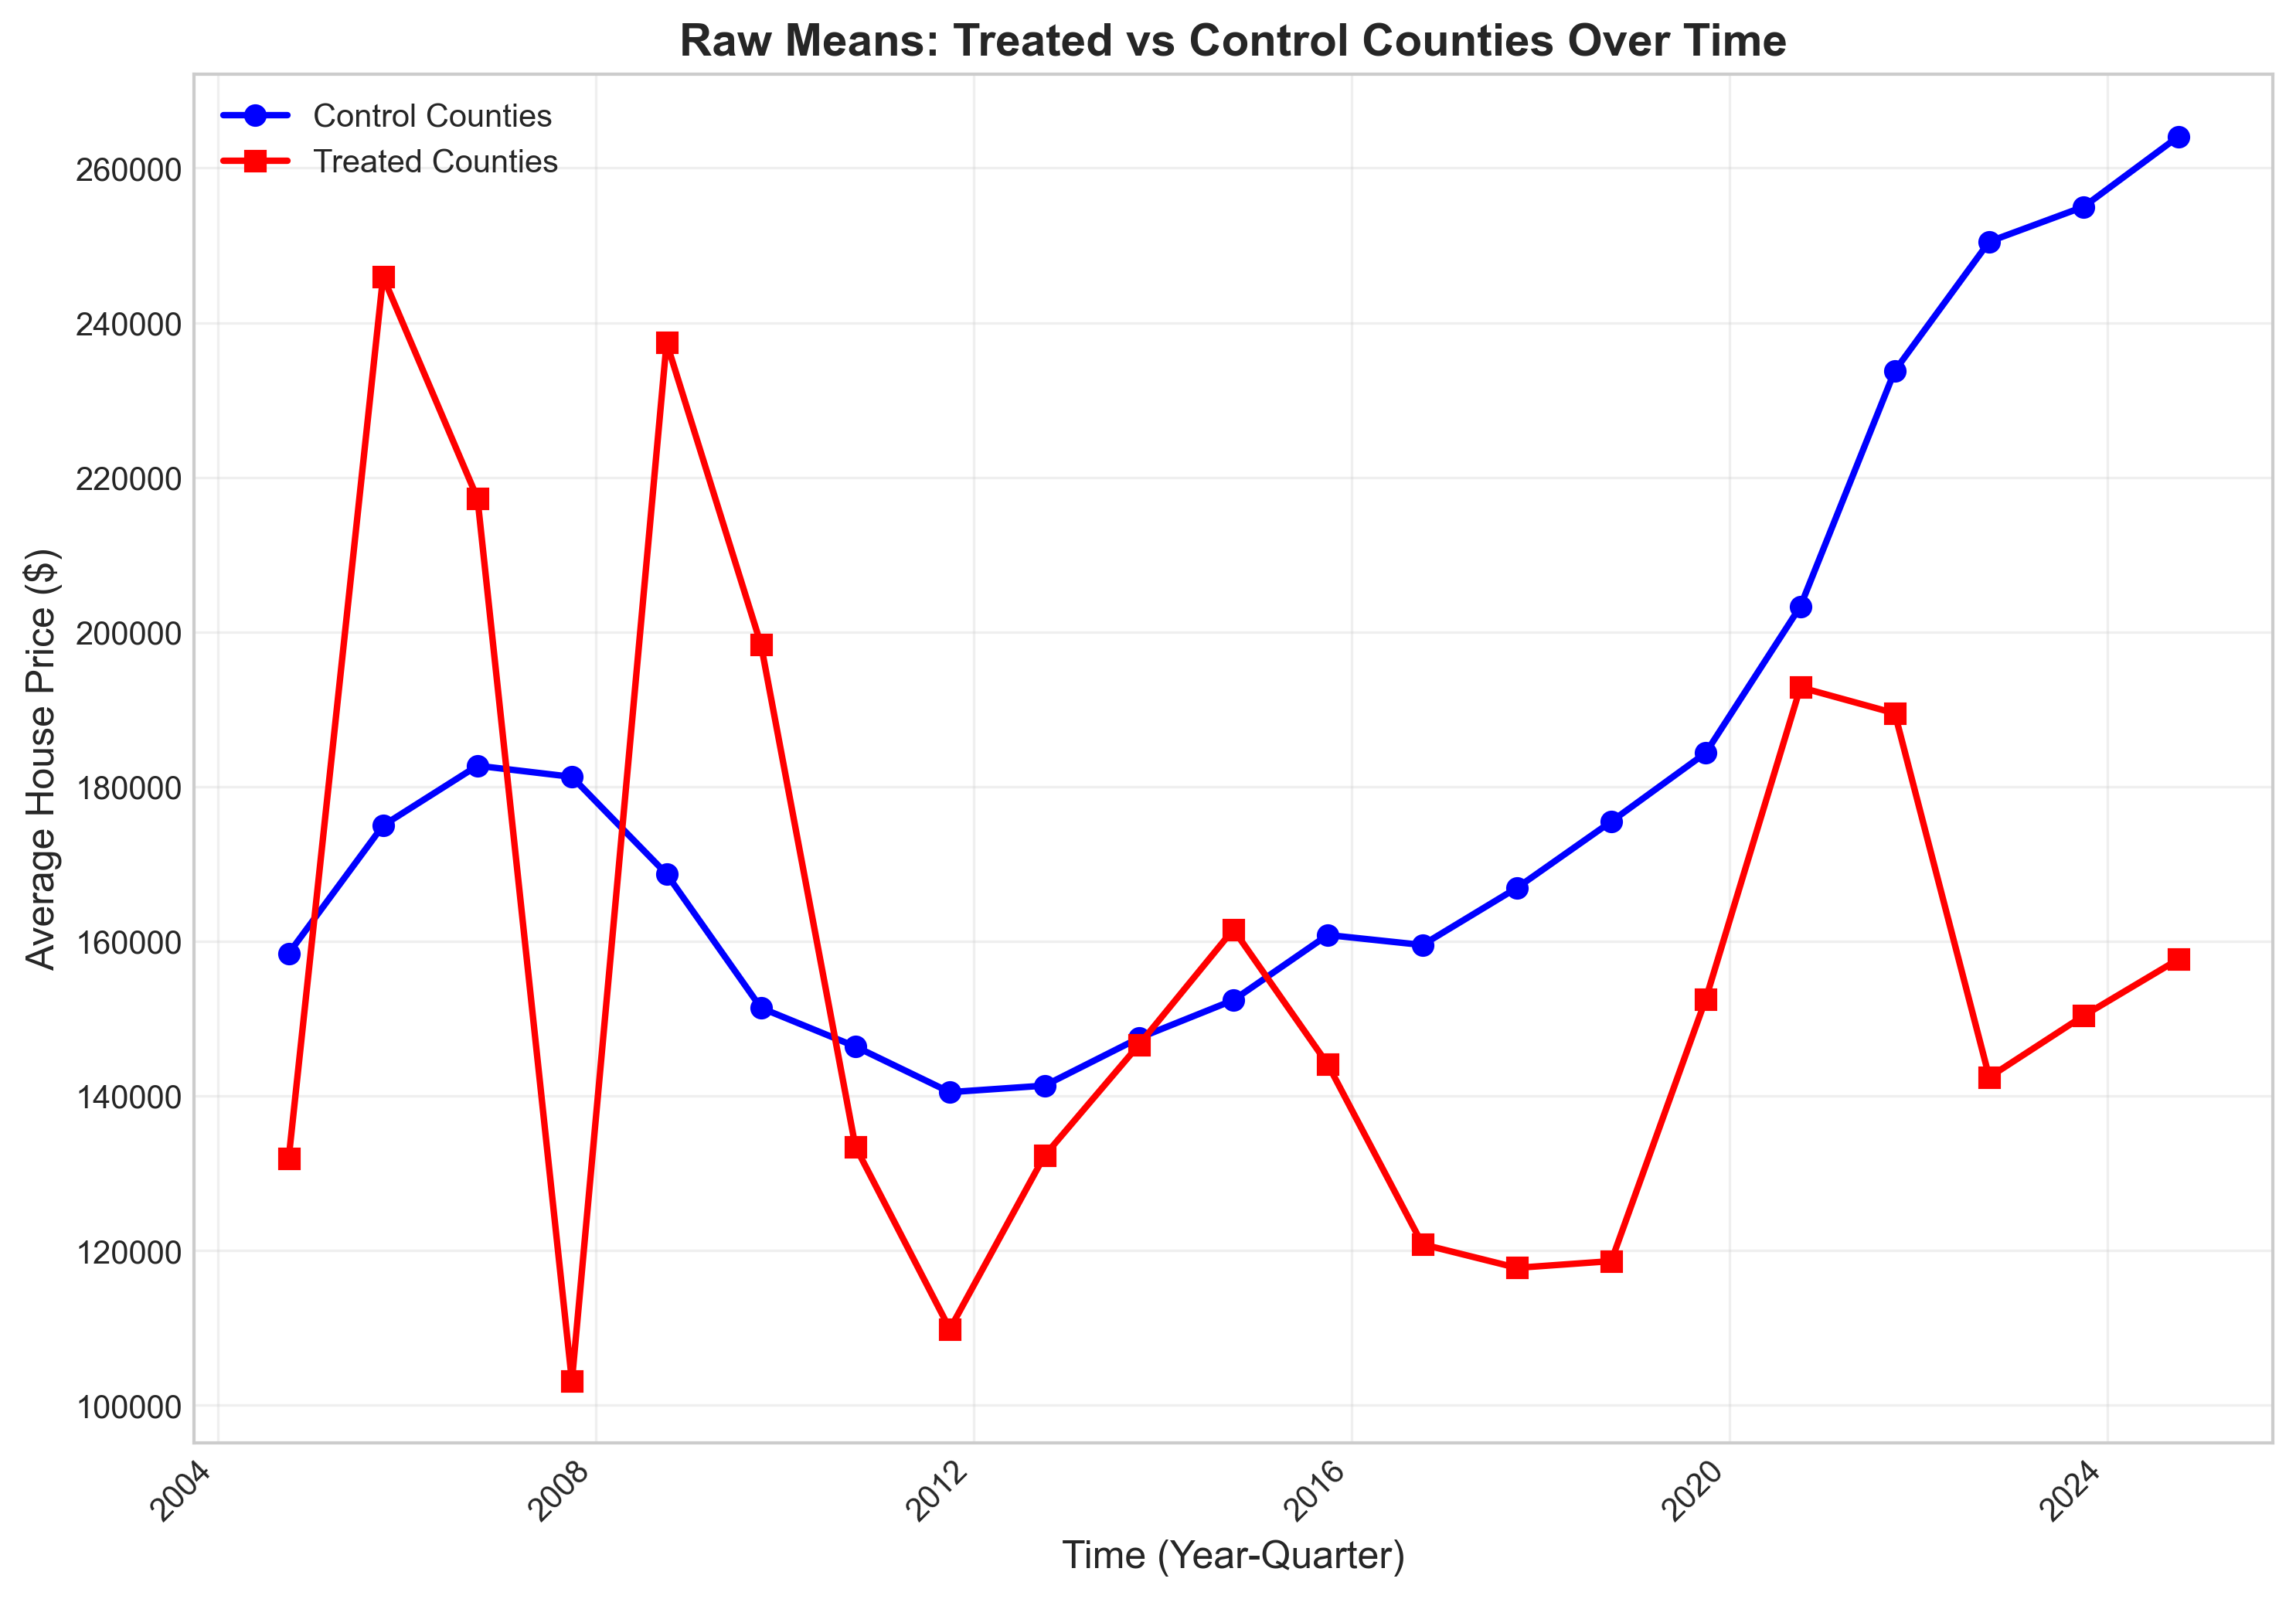
\includegraphics[width=0.96\textwidth]{raw_means_plot.png}
    \caption{Simple mean across counties of Zillow Home Value Index, by quarter, for treated and control counties. The treated counties are those that experienced exactly one hospital closure during the sample period. The control counties that never experienced any hospital closure during the sample period.}
    \label{fig:rawmeans} 
\end{figure}
\newpage
\section{Literature}

\citep{BadillaMarotoFaberLevyMunoz2024} seems closest to the topics I'm interested in. They find a positive impact on housing prices. One of their main findings is shown in Fig. \ref{fig:retiree_share_france}.

\begin{figure}[htbp]
    \centering
    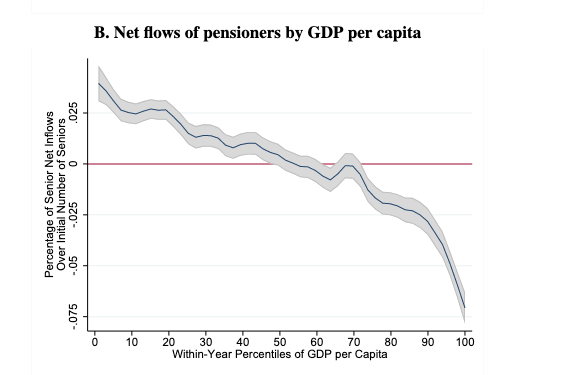
\includegraphics[width=\textwidth]{munoz.png}
    \caption{Negative correlation between GDP per capita and inflows of seniors}
    \label{fig:retiree_share_france}
\end{figure}

%Some mechanisms explored are homophily / taste for retiree communities.  


They use French data because it has microdata on migration flows since 1962, containing ``individual-level information on precise residence location, age, marital status,  occupation and housing status, and mobility since the last Census wave.''


What I hope to do differently is show specific mechanisms determining senior migration choice, such as presence of healthcare or cost-of-living, and perhaps endogenize choices by local governments to make themselves more or less attractive to retirees (this paper is very reduced-form).
\bibliography{references}
\end{document}